\documentclass[11pt,a4paper,BCOR10mm,bibtotocnumbered]{scrbook}

%% \usepackage{abstract}          % typesetting of a abstract environment

\usepackage{acronym}          % acronyms
\usepackage{amscd}            % Kommutative Diagramme
\usepackage{amsmath}          % mathematics
\usepackage{amsfonts}         % mathematics
\usepackage{array}            % tabels
\usepackage{fancyvrb}         % Umgebung f�r Programm-Listings
\usepackage{float}            % mehr Positionen von Float-Umgebungen
\usepackage[T1]{fontenc}      % Fonteinstellung
\usepackage{graphicx}         % Laden von Bildern
%\usepackage{glossary}         % Erstellen eines Glossars DONT EVER USE THIS
\usepackage[nonumberlist]{glossaries}
\usepackage{hyperref}         % Querreferenzen und Links
\usepackage[latin1]{inputenc} % Zeichenkodierung
\usepackage{keystroke}        % Tastendarstellung
\usepackage{lscape}           % Landscape 
\usepackage{makeidx}          % Indexerstellung
\usepackage{mflogo}           % LaTeX-Logos
\usepackage{multicol}         % mehrspaltiger Satz
\usepackage{multirow}
\usepackage[numbers]{natbib}  % Autor-Datum Zitierungen
%\usepackage{ngerman}          % Zur Verwendung der deutschen Sprache
\usepackage{rotating}         % Rotieren von Bildern und Texten
\usepackage{syntax}           % Syntax-Diagramme
\usepackage{typearea}         % Satzspiegelberechnung
\usepackage{url}              % Hyperlinks
\usepackage{xspace}           % Korrekter Leerraum nach Befehlen
\usepackage{listings}         % Auflistung von Ausschnitten von Programm-Code
\usepackage[T1]{fontenc}      % ben�tigt von luximono
\usepackage{subfigure}        % Unterabbildungen
\usepackage{textcomp}         % Verschiedene Zeichen im textmode
\usepackage{xcolor}
\usepackage{courier}
 


\usepackage[bachelorproject,english]{rtsstud}          % Lehrstuhl-Spezifikationen
\usepackage{rtsabstr}         % Zusammenfassung

\graphicspath{{pictures/}}
  
\newcommand{\listingxml}{
\lstset{
basicstyle=\scriptsize\tt,
numbers=left,
frame=shadowbox,
tab=.,
language=XML,
tabsize=2,
showspaces=false,
showstringspaces=false,
captionpos=b,
basicstyle=\footnotesize,
backgroundcolor=\color[rgb]{1,1,0.74},
keywordstyle=\tiny\bfseries,
numbers=left,
numberstyle=\tiny,
numberblanklines=false,
}}
\newcommand{\listingjava}{
\lstset{
basicstyle=\scriptsize\tt,
numbers=left,
frame=shadowbox,
tab=.,
rulesepcolor=\color{lightgray},
morecomment=[l]{//},
tabsize=3,
language=Java,
keywordstyle=\bfseries\color[rgb]{0.482,0,0.323},
stringstyle=\color{blue},
commentstyle=\color[rgb]{0.224,0.49,0.353},
numberstyle=\tiny,
breaklines=true,
showstringspaces=false,
showtabs=false,
showspaces=false,
backgroundcolor=\color[rgb]{1,1,0.74},
emph={},
emphstyle=\bfseries\color[rgb]{0.482,0,0.323}
% frame=single, %single
% backgroundcolor=\color[rgb]{1,1,0.6}
}}

\newcommand{\showlistingex}[5]{
\begin{figure}[#5]
{
% \hspace{0.4cm}
\scriptsize
\lstinputlisting[language=#2,label=#4,caption=#3]{#1}
\normalsize
% \hspace{0.1cm}
}
\end{figure}
}



\title{Configurations and Automated Execution in the KIELER Execution Manager}
\subtitle{~}
\author{cand.~inform.~S\"oren Hansen}
\date{\today}
\advisor{%
  \renewcommand{\thefootnote}{\fnsymbol{footnote}}%
  Christian Motika\\
}

% {%
% \renewcommand{\thefootnote}{\fnsymbol{footnote}}
% \protect\footnotemark
% \footnotetext[1]{Das ist eine Anmerkung zur Person.}
% }

\makeindex


\begin{document}

\frontmatter
\maketitle
\assertion
% \begin{abstract}
Execution Manager is used in KIELER as a framework to plug-in DataComponents for various tasks. Examples are:
\begin{itemize}
 \item Simulation Engines
 \item Model Visualizers
 \item Environment Visualizers
 \item Validators
 \item User Input Facilities
 \item Trace Recording Facilities 
\end{itemize}

These DataComponents can be executed using a graphical user interface (GUI). 
The scheduling order can also be defined by this GUI as well as other settings like a step/tick duration and properties of DataComponents.

In order to make it more comfortable for the user, preference pages for the Execution Manager could offer the following:
\begin{itemize}
 \item Configure a default configuration
 \item Including timeouts, debug level, scheduling, other settings
 \item Make these things specific for a diagram type
 \item Provide a mechanism to access some last used configurations/schedules 
\end{itemize}

For information about KIEM see - http://rtsys.informatik.uni-kiel.de/trac/kieler/wiki/Projects/KIEM

\end{abstract}


\makeatletter
\@ifundefined{float@listhead}{}{%
    \renewcommand*{\lstlistoflistings}{%
        \begingroup
    	    \if@twocolumn
                \@restonecoltrue\onecolumn
            \else
                \@restonecolfalse
            \fi
            \float@listhead{\lstlistlistingname}%
            \setlength{\parskip}{\z@}%
            \setlength{\parindent}{\z@}%
            \setlength{\parfillskip}{\z@ \@plus 1fil}%
            \@starttoc{lol}%
            \if@restonecol\twocolumn\fi
        \endgroup
    }%
}
\makeatother


%% Inhaltsverzeichnis
\tableofcontents

%% Inhaltsverzeichnis
\listoffigures

%% Verzeichnis der Auflistungen
\lstlistoflistings

%% Inhaltsverzeichnis
\listoftables

%% Verzeichnis der Abk�rzungen

%% Abbreviations
\chapter*{Abbreviations}
\begin{acronym}
 \acro{API}{Application Programming Interface}
 \acro{CSV}{Comma-Separated Values}
 \acro{GUI}{Graphical User Interface}
 \acro{IDE}{Integrated Development Environment}

 \acro{KIEL}{Kiel Integrated Environment for Layout}
 \acro{KIELER}{Kiel Integrated Environment for Layout Eclipse Rich Client}
 \acro{KIEM}{KIELER Execution Manager}
 \acro{KIEMAuto}{Automated Executions for the KIEM}
 \acro{KIEMConfig}{Configurations for the KIEM}
 \acro{KIML}{KIELER Infrastructure for Meta Layout}
 \acro{KSBasE}{KIELER Structure Based Editing}

 \acro{OS}{Operating System}
 \acro{RCA}{Rich-Client Application}
 \acro{UI}{User Interface}
 \acro{XML}{Extensible Markup Language}
\end{acronym}


%%% Local Variables: 
%%% mode: latex
%%% TeX-master: "paper"
%%% End: 


%% Verzeichnis der Akronyme
% 
\chapter*{Verzeichnis der Akronyme}
\begin{acronym}[KIEL]
 \acro{KIEL}{Kiel Integrated Environment for Layout}
\end{acronym}

%%% Local Variables: 
%%% mode: latex
%%% TeX-master: "paper"
%%% End: 


%%% Local Variables: 
%%% mode: latex
%%% TeX-master: "paper"
%%% End: 
% 
\chapter*{Verzeichnis der Akronyme}
\begin{acronym}[KIEL]
 \acro{KIEL}{Kiel Integrated Environment for Layout}
\end{acronym}

%%% Local Variables: 
%%% mode: latex
%%% TeX-master: "paper"
%%% End: 


\mainmatter

% \part{Erster Teil} % Teile nur bei sehr langen Arbeiten

\chapter{Introduction}
\label{chapter:introduction}
\section{KIELER Framework}
\label{sec:intro/Kieler}
\begin{itemize}
 \item layouter, structure based editing
 \item syncharts
 \item simulater
 \item execution manager
\end{itemize}
\section{The KIELER Execution Manager}
\label{sec:intro/Kiem}
Execution Manager is used in KIELER as a framework to plug-in DataComponents for various tasks. Examples are:
\begin{itemize}
 \item Simulation Engines
 \item Model Visualizers
 \item Environment Visualizers
 \item Validators
 \item User Input Facilities
 \item Trace Recording Facilities 
\end{itemize}

These DataComponents can be executed using a graphical user interface (GUI). 
The scheduling order can also be defined by this GUI as well as other settings like a step/tick duration and properties of DataComponents.
For information about \ac{KIEM} see the wiki\footnote{\url{http://rtsys.informatik.uni-kiel.de/trac/kieler/wiki/Projects/KIEM}}.
\section{Outline of this Document}
\label{sec:intro/Outline}
The first part of this document is about the implemention of the Configuration plugin for the \ac{KIEM}.
The second part discusses the implementation of the Automated Execution plugin for the \ac{KIEM}. Both
parts will have the same structure described below.
Each part starts with a detailed outline of the problems that are to be solved by this thesis.
The next section introduces technologies used to solve the problem.
After that there will be a section about the concepts of how to solve the problem and some
design decisions that were made at a very early stage in the development.
Sections 5 and 6 are about the actual implementation with section 5 outlining the changes
that were made to the \ac{KIEM} plug-in itself and section 6 describing the newly created
\ac{KIEMConfig} plug-in.
The final section of each part will summarize the results of the thesis and outline
a few projects that could be based on it.







%%% Local Variables: 
%%% mode: latex
%%% TeX-master: "paper"
%%% End: 



\part{Configuration Management}
\chapter{Used Technologies}
\label{chapter:ConfTechnology}
Before the problem can be explained the technologies in question
and the terminology that is used in the rest of this document is in order must first be introduced. This should
only serve as a brief outline since a full explanation goes beyond the scope of this thesis.

In addition to these technologies a section about some related work is included in this chapter.

\section{Eclipse}
\label{section:ConfTechEclipse}
\index{Eclipse}
Since the \ac{KIELER} project and thus the Execution Manager is build upon the 
Eclipse framework a short introduction into Eclipse is necessary.

The basic function of Eclipse is as \textit{the} \ac{IDE} for Java. It provides
a host of facilities that makes it easier for the user to create their own Java Applications.
A few examples for these facilities are:
\begin{itemize}
 \item Syntax highlighting to make the source code easier to read.
 \item Automatic completion of partial commands to ensure correctness
and make it easier to write code.
 \item Content assist to create better code and remove errors.
 \item Several wizards for class creation and other tasks.
\end{itemize}

However since Eclipse is an open-source project there are also plug-ins\footnote{Section 
\ref{section:ConfTechPlugins}} for variety of other things. 
For example the language isn't limited to Java. There are also plug-ins
for C++, \LaTeX, Visual Basic and several other programming languages.

Through the use of different modeling framework Eclipse can also be used as an \ac{IDE}
for \ac{IDE}s. That makes Eclipse ``an IDE for anything, and nothing in particular'' \cite{eclipseOverview}.

\begin{figure}
  \centering
  \includegraphics[scale=.25]{EclipseScreen.png}
  \caption[The Eclipse workbench window]%
  {The Eclipse workbench window\protect}
  \label{fig:EclipseScreen}
\end{figure}
The terminology used for the different basic parts of Eclipse can be illustrated based on Figure
\ref{fig:EclipseScreen}:
\begin{itemize}
 \item The main window of Eclipse is called the \textit{workbench}. The workbench consists of the 
different editors and views.
 \item The files that the user operates on are located in the Eclipse \textit{workspace}. 
 \item An \textit{editor} is a component that allows the user to display, enter and modify information.
Editors are used to modify a specific file type. There can usually be multiple instances of the same editor.
An example for an editor would be the Java Editor which is used to create and edit Java Source Files.
 \item An Eclipse \textit{view} is the other component located on the workbench. Views are only used to
display content that was created elsewhere. Unlike editors there is usually only one instance of any view.
One of the views shown in the figure is the class outline view. It shows all methods and attributes of the 
Java class in the currently active editor.
\end{itemize}

For additional information about Eclipse see the official Eclipse website\footnote{www.eclipse.org} or literature \cite{eclipsePlugins}.

\subsection{Plug-ins}
\label{section:ConfTechPlugins}
\index{Plug-in}
The building blocks of any Eclipse application are the so called \textit{plug-ins}. They
consist of any number of Java classes and additional meta information. The Java classes
describe the behavior of the plug-in and define its \ac{API}. The meta information is not written
in Java but uses an \ac{XML}\footnote{\url{http://www.w3.org/XML/}} notation instead. The meta information contains the following
information:
\begin{itemize}
 \item What other plug-ins does the plug-in depend on? This information is necessary to determine
which other plug-ins have to be loaded or when to refuse loading the plug-in because of missing
dependencies.
 \item What \textit{extension points} does the plug-in offer? These are part of the \ac{API} and
will be described below.
 \item What functionality does it add to the plug-ins which it extends?
\end{itemize}

Plug-ins encapsulate their internal behavior and can be accessed through the \ac{API} and the 
\textit{extension points}. They provide a specific functionality that can be reused as long as
the dependencies are met. As such an Eclipse application consists of a mosaic of different
plug-ins that can be exchanged at will.

Eclipse can not only be used to create plug-ins that can be used in an Eclipse
instance but can also compile a set of plug-ins into a standalone application - the so
called \ac{RCA}\footnote{\url{http://wiki.eclipse.org/index.php/Rich_Client_Platform}}. 
This \ac{RCA} contains a minimal set of plug-ins to provide the Eclipse
look-and-feel and the plug-ins created by the user.

\subsubsection{Extension Point Mechanism}
\label{section:ConfTechExtension}
\index{Extension point}
The extension point mechanism is one of the key features of plug-in development in Eclipse.
It extends the \ac{API} provided by the public methods of the different Java classes inside
the plug-in. An extension point definition consists of a tree of different configuration elements.
Each configuration element has different attributes some of which can be optional while other
are mandatory. These attributes can be anything from a String, a file to a Java class that has
to extend one class and implement a specific interface.

A plug-in that wants to add their functionality to an already existing plug-in
through the use of an extension point has to provide the mandatory attributes defined in the 
specifications.

Eclipse itself already provides many extension points to extend the functionality of the workbench.
For example, if a plug-in wants to add a new editor to the workbench it has to extend the 
\textit{org.eclipse.ui.editors} extension point. It then has to provide an identifier and a name
as well as a class that implements the \textit{org.eclipse.ui.IEditorPart} interface. It can also specify an
icon and a file extension for files which should be opened with the new editor.

When an Eclipse application is started with this plug-in Eclipse will automatically make sure that the new editor
can be used to open the specified file type. The programmer only has to concern himself with the area of the editor
itself without worrying about it being added at all the necessary places inside the Eclipse architecture.

\subsection{Preference Pages}
\label{section:TechPreferencePage}
\index{Preference Page}
\begin{figure}
  \centering
  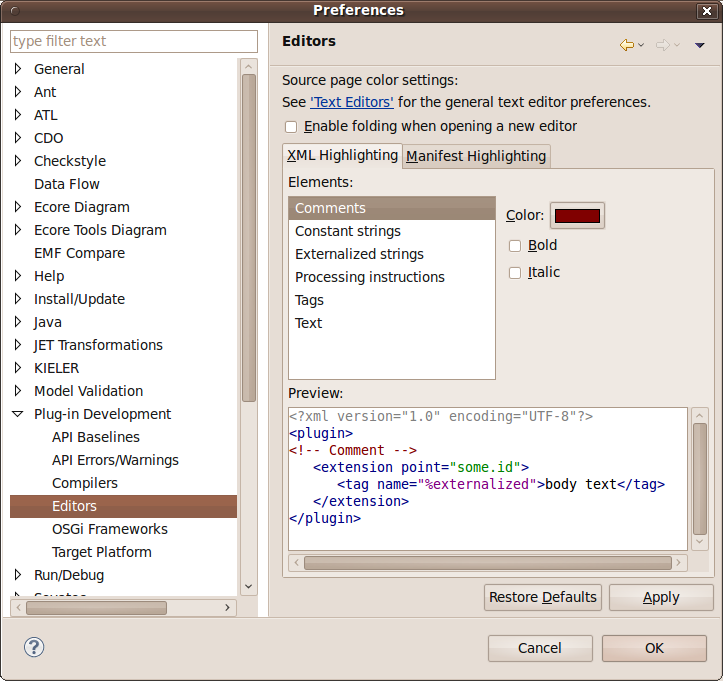
\includegraphics[scale=.3]{PreferencePage.png}
  \caption[An example for a preference page.]%
  {An example for a preference page.\protect}
  \label{fig:PreferencePage}
\end{figure}
A special example of plug-in usage within the Eclipse framework itself is the 

\textit{org.eclipse.ui.preferencePage} plug-in. 
It is used to create new preference pages\footnote{Figure \ref{fig:PreferencePage}}
at a specific location inside the normal tree of preference pages accessible through Window->Preferences.
The programmer only has to take care of the contents of the actual page and not worry
about additional buttons or integrating it into the PreferenceDialog.

\subsubsection{Preference Store}
\label{section:TechPreferenceStore}
Closely coupled with the preference pages is the Eclipse preference store. It is
basically a text file for each plug-in where the plug-in can deposit simple Strings
under a given key to ensure that information is kept between execution runs. For
an example of the use of the preference store see Listing \ref{list:AppendixSavedConf}
in the Appendix.

\section{The KIELER Execution Manager}
\label{section:introKiem}
\index{Execution Manager}
\begin{figure}
  \centering
  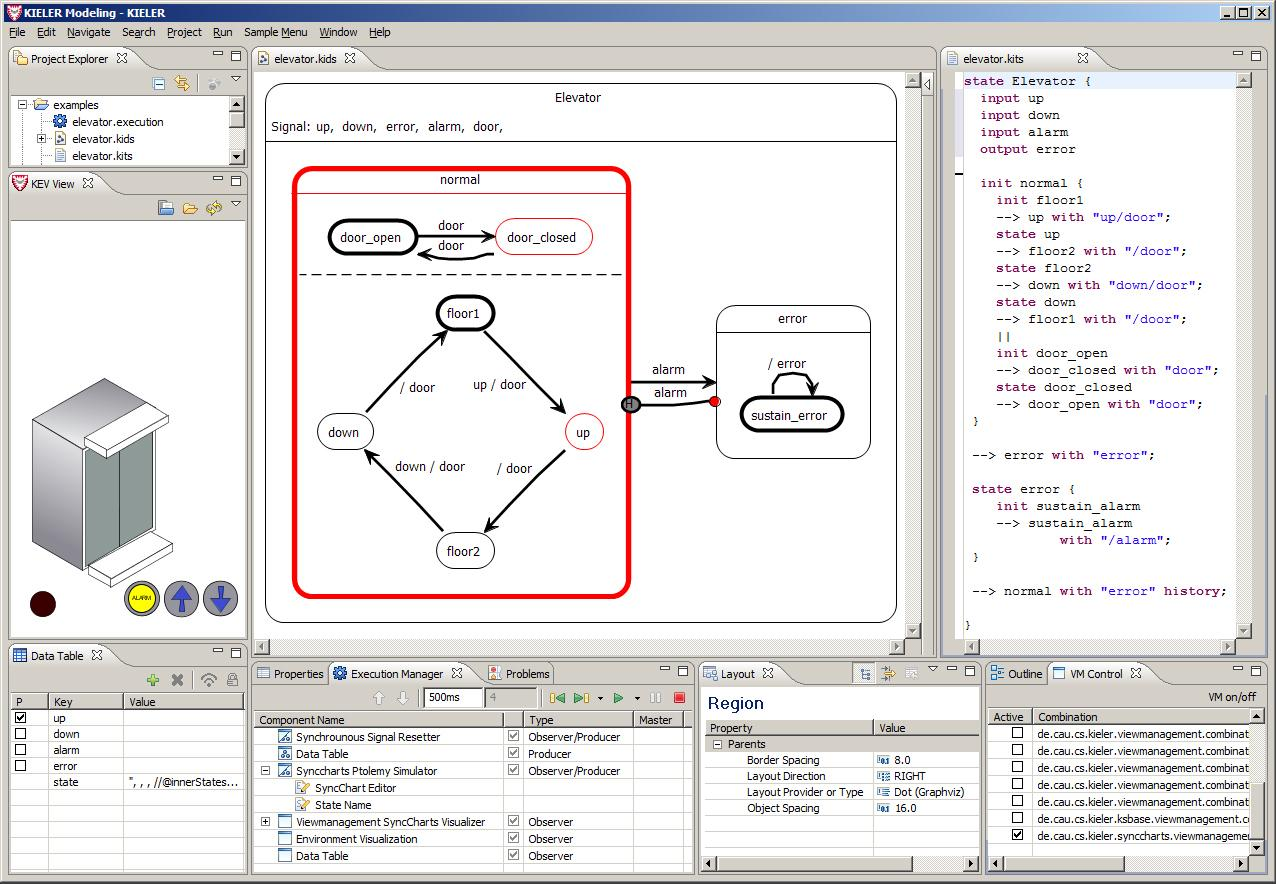
\includegraphics[scale=.3]{KIEMOriginal.jpeg}
  \caption[The Execution Manager during a simulation.]%
  {The Execution Manager during a simulation. [image taken from \cite{cmot-dt}]\protect}
  \label{fig:KIEMOriginal}
\end{figure}

Execution Manager shown in Figure \ref{fig:KIEMOriginal} is used in \ac{KIELER} as a framework 
to plug-in DataComponents\footnote{Section \ref{section:IntroDataComponent}} for various tasks. Examples are:
\begin{itemize}
 \item Simulation Engines
 \item Model Visualizers
 \item Environment Visualizers
 \item Validators
 \item User Input Facilities
 \item Trace Recording Facilities 
\end{itemize}

These DataComponents can be executed using a graphical user interface (GUI). 
The scheduling order can also be defined by this GUI as well as other settings like a step/tick duration and properties of DataComponents.
For information about \ac{KIEM} see the wiki\footnote{\url{http://rtsys.informatik.uni-kiel.de/trac/kieler/wiki/Projects/KIEM}}.

\subsection{KiemProperty}
\label{section:IntroKiemProperty}
The basic KiemProperty object holds a (key, value) pair of type String. It is used to store information
inside the DataComponents. There are also advanced KiemProperties which can contain other types of values
like integers, booleans or files.

\subsection{DataComponents}
\label{section:IntroDataComponent}
\index{DataComponent}
A DataComponent is an entity that has a specific task during a the course of an execution. The
DataComponents are scheduled in a specific order and can either receive or produce information or both. 
During each step of the execution each DataComponent is asked to perform their computations for the step. Every
DataComponent contains a list of KiemProperties that are used to allow some configuration of the component
after it has been loaded.

\subsubsection{DataComponentWrappers}
\label{section:IntroDataComponentWrapper}
\index{DataComponentWrapper}
A DataComponentWrapper is an object that wrapps around a DataComponent. The wrappers are stored in the schedule
of an execution file.

\subsection{Execution}
\label{section:IntroExecution}
\index{Execution file}
\index{Execution}
\index{Schedule}
The files used by the Execution Manager are called \textit{execution files}. These files contain 
the list of DataComponents with all internal data and the specific order. That list is called a
\textit{schedule}. The schedule can be used to start an \textit{execution} in the Execution Manager.
An execution consists of a initialization, stepping and wrap-up.

\subsection{Model Files}
\label{section:IntroModelFile}
\index{Model file}
\begin{figure}
  \centering
  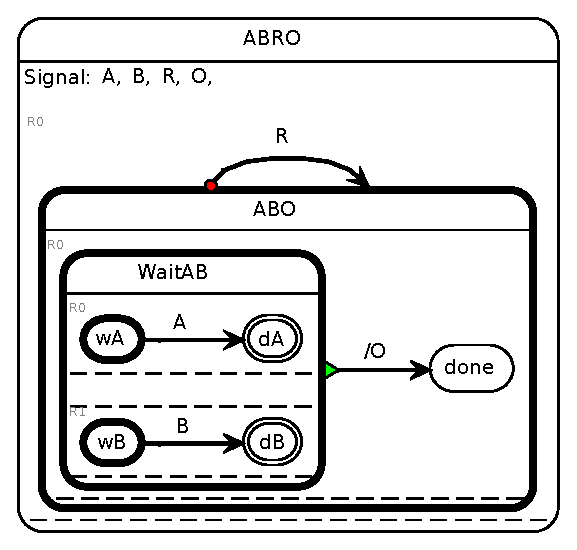
\includegraphics[scale=.9]{abro.pdf}
  \caption[An example for a simple syncchart diagram.]%
  {An example for a simple syncchart diagram.\protect}
  \label{fig:abro}
\end{figure}
A model file is not a concept of the Execution Manager as such but rather a general concept. However
since this thesis only uses model files in the context of the \ac{KIEM} it seems appropriate to explain
them here.

A model file can be any file that contains the structure and behavior of a semantic entity. This can be something as
simple as a text file containing a list of elements in a certain order. Most model files that are used in
the \ac{KIELER} project are diagrams that consist of nodes and links. These \textit{synccharts} are build in
a hierarchical structure and are therefore stored as a tree of different elements. An example for a simple
syncchart diagram is shown in Figure \ref{fig:abro}.

\section{Related Work}
\label{section:RelatedWork}
There are of course a huge amount of other applications and projects that deal
with configuration management. In order to get some idea of similar projects
a few examples from Eclipse itself and the \ac{KIELER} project will be used.

\subsection{Configurations}
\label{section:RelatedConf}
\index{Configuration}
One of the tasks that will be explained in Section \ref{section:ConfTaskConfig} is to add new
configuration information to existing execution files. This task can be compared to
the \ac{KIML} project. 

\ac{KIML} is used to automatically layout existing diagrams. Since diagrams basicly consist of nodes and
connections generic algorithms can be used to layout almost any type of diagram. However the user still
has some control over the details of the automatic layout process. The user can configure details like
the distance between different elements, the direction of the layout or the layouter that should be used.

This meta-information has to be stored somewhere. The approach used in \ac{KIML} was to create a separate
file. The file has the same name as the diagram file and contains all the layout information needed for it.
The information can be easily reset by deleting the separate file. 

\chapter{Problem Statement}
\label{chapter:ConfTask}
The objective of this project is to improve the configurability of the
Execution Manager as outlined in the diploma-thesis by Christian Motika\cite{cmot-dt} :
\begin{quote}
 \ac{KIEM} currently does not have a preference page to save
additional settings like DataComponent timeouts. Also execution schedulings
might be similar for a common diagram type.

It may improve the usability further to allow the user to customize execution
schedulings for specific diagram types. An interface for these kind of settings
could be realized as an Eclipse preference page.
\end{quote}

This task will be explained in more detail in this chapter. It will start by introducing 
solutions to the problem of how to save the new configuration properties into the existing 
execution files. In addition the chapter will explain ways to enable the user to set up a 
series of default configurations. The last section of this chapter will explore 
possibilities of how to make it easier to load previously saved schedules.

\section{Configurations}
\label{section:ConfTaskConfig}
\index{Configuration}
Currently every property in the Execution Manager has a hard coded default value. There is a text box
for setting the aimed step duration for the currently loaded execution file but that value
is lost once a new execution file is loaded.
To solve this problem an extension to the Execution Manager should attempt to provide the following:
\begin{enumerate}
 \item Find a way that execution files can store values like the aimed step duration and the timeout.
This mechanism should be implemented in a way that ensures that old files can be upgraded and new
files are still valid in instances of the Execution Manager that don't use the configuration plug-in.
 \item Find a way to load the configurations into the different parts of the Execution Manager as soon as an
execution file is loaded from the file system.
 \item Ensure that the user can edit all properties and maybe even create his own custom properties.
This should be implemented in a way that doesn't clutter up the current user interface too much.
\end{enumerate}

\subsection{Default Configuration}
\label{section:ConfTaskDefaultConfig}
\index{Default Configuration}
The different properties stored in each execution file might sometimes not suit the users current needs
and he might want to use a default value for some properties without having to manually set them
in each new configuration.
The solution could be implemented using the preference mechanism provided by Eclipse.
\begin{enumerate}
 \item There should be a way to set the default properties for all Execution Manager properties 
and possibly for user defined properties as well.
 \item It should be possible for the user to set up which of these properties should override 
the value stored in the execution file and which should only be used if the execution file doesn't contain one.
\end{enumerate}

\section{Easier Schedule Loading}
\label{section:ConfTaskEasyLoading}
The last objective of this thesis is to make it easier to load execution files.
Currently all execution files are stored in the workspace at a place of the users choice. In a very
large workspace it can be very hard to find the execution file that you need for your current
simulation. The list of recently used documents provided by Eclipse is of little use since all
opened documents are placed there, not just execution files.
This problem leads to the following tasks:
\begin{enumerate}
 \item Finding a way to track recently used execution files and make it easier for the user to
load them without the need to locate them inside his workspace.
 \item In addition to tracking recently used execution files the user might want to have a way to get a list
of execution files that work for the currently active editor. This list should be sorted with the most likely
candidates at the top to allow less experienced users to select an execution file that will most likely work.
\end{enumerate}

\chapter{Concepts}
\label{chapter:ConfConcepts}
The solution to the problems outlined in chapter \ref{chapter:ConfTask} can be achieved with
the help of the Eclipse plug-in technology described in chapter \ref{chapter:ConfTechnology}.

\section{Configurations}
\label{section:ConfConceptsConf}
The first approach to save additional configuration information in the execution files would
be to actually modify the format of those files and write the information into them.
This would most likely be the easiest approach but would destroy backward compatibility of
those files since the basic \ac{KIEM} would not know how to deal with the modified files.

The approach taken in this thesis is based on the list of DataComponents. Each execution file 
carries a list of its own DataComponents and their properties to ensure
that the component are properly initialized the next time the execution is loaded. That list
can be loaded even if there are DataComponents contained in it that are not present in the current
runtime configuration. The \ac{KIEM} will show a warning indicating that it doesn't know the given
component but proceed toload the rest of the execution. 

These DataComponents basically just carry a list of KiemProperties which are
basically (key, value) pairs. Hence, they are suited well for storing simple information like the value
of a text field.

To solve the problem a new type of DataComponent will have to be constructed and registered through
the extension point in the \ac{KIEM}. This ensures that the component can be added to any execution
file. The \ac{KIEM} ensures that all properties contained in our component will be saved with
the execution file and loaded the next time the file is opened. After that the configuration plug-in has 
find the component inside the DataComponent list, get the properties saved inside it
and set them inside the \ac{KIEM}.

% \begin{itemize}
%  \item .execution files carrying list of DataComponents, add configuration component
% automatically saved with file, doesn't break old files, new files are still
% can still be loaded without the plug-in
%  \item configurations saved anyway through the saveble view
% \end{itemize}

\subsection{Default Configuration}
\label{section:ConfConceptsDefaultConf}
\index{Default Configuration}
In order to provide a place to manage the default configurations we will be
using the Eclipse preference pages.

The root page for the \ac{KIEM} should contain the basic KIEM properties like
the aimed step duration, timeout and the view elements of the Configuration
plug-in.

\begin{figure}[MSPLayoutPreferencePage]
  \centering
  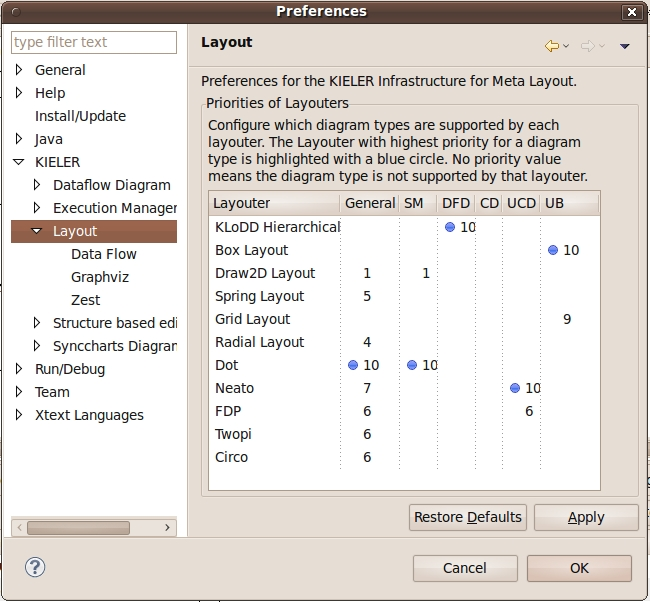
\includegraphics[scale=.5]{MSPLayoutPreferencePage.jpg}
  \caption[Layout Preference Page by Miro Sp\"onemann]%
  {Layout Preference Page by Miro Sp\"onemann\protect\footnotemark}
  \label{fig:MSPLayoutPreferencePage}
\end{figure}

Then we will construct another page for managing the different schedules
and their editors. For that we will adapt the LayoutPreferencePage by Miro Sp\"onemann
as seen in Figure \ref{fig:MSPLayoutPreferencePage} where we will just replace the 
layouts with the list of registered schedules.

For the purpose of sorting the schedules that match the currently opened editor they will
need to have user defined priorities which can be easily set up with the table
shown above.

The last page will be used to allow the user to set up his own properties and give them
default values.

The values entered in those pages will be stored inside the Eclipse Preference
Store.

%\begin{itemize}
% \item eclipse preference page architecture
% \item plug into KIELER preference page tree, create series of elements to
% configure item that are now only configurable through KiemView 
% \item use eclipse preference store to save values
% \item multiple pages for different aspects, user friendly, easier to maintain
%\end{itemize}

\section{Easier Configuration loading}
\label{section:ConfConceptsEasyLoading}
For easier configuration loading we will add two ComboBoxes to the existing
tool bar inside the \ac{KIEM} view.

One of them will display the list of recently used schedules the other one the
list of schedules that work for the currently active editor.

As soon as the user opens a new execution file through the normal workspace
view we will be notified of that event by the \ac{KIEM}. We will then create a new
schedule and store the path to the execution file in it along with the editor
that was opened at the time that the schedule was created. The new schedule will
also be added to the list of recently used schedules that we maintain through the 
use of the Eclipse preference store.

When the user selects one of the previously saved schedules in one of the
ComboBoxes we will retrieve the saved path and offer it to the KiemPlugin to
load it in the hopes that the execution file is still in the same location and
wasn't deleted, renamed or moved by the user.

% \begin{itemize}
%  \item keep a list of recently opened schedules in the preference store
%  \item allow access to that list through either menus or the KIEM itself
%  \item pass the saved path to KIEMPlugin to load it
%  \item store a list of editors that work for each .execution file together with their path
%  \item determine which editor is open and find matching files
% \end{itemize}
\chapter{Code Changes in the Execution Manager}
\label{chapter:KiemChanges}
Although the project attempts to realize most of the objectives without
changing the Execution Manager itself minimal adaptations were necessary.
This mostly involves adding new methods to the \ac{API} in order to
gain access to previously hidden properties.

Also some changes had to be performed where properties were loaded from hard-coded 
default values. These were refined and will now only be used if the \ac{KIEMConfig} 
plug-in is not registered to supply previously saved properties.

However all changes that were made to the \ac{KIEM} plug-in were merely additions
and won't break any plug-ins relying on the old implementation.

\section{Schema Files and Interfaces}
\index{Extension point}
In order to provide additional functionality for other plug-ins we choose the extension
point mechanism described in Section \ref{section:ConfTechExtension}. This is done
is order to retain the old functionality of the plug-in while on the other hand giving
options to ask extending plug-ins for their contributions. 

The extension points are described in more details in the next sections. They consist
of a schema file for defining the extension point and an interface that contains the 
methods that extending components have to supply.

\subsection{Toolbar Contribution Provider}
\label{section:ToolbarContributionProvider}
\index{Toolbar Contribution Provider}
The purpose of the tool bar contribution provider is to allow other plug-ins to put
items onto the tool bar of the Execution Manager. 
There are two reasons for using the extension point mechanism
rather than making the tool bar available and have other plug-ins put their
contributions directly on it:
\begin{enumerate}
 \item At the moment the tool bar and all contributions are created dynamically. Switching
the entire native tool bar of the Execution Manager to adding the actions to the tool bar
through a predefined Eclipse extension point would require major code changes and
have major drawbacks.
 \item A programmatic approach gives control over the contributions to the Execution Manager.
This means that the order of the native Execution Manager buttons is always the same and in the
same place. It also means that the Execution Manager can choose to ignore contributions if the
tool bar gets too crowded.
\end{enumerate}
\listingjava
\showlistingex{code/IKiemToolbarContributor.txt}
{Java}
{The interface for ToolbarContributionProviders}
{list:IToolbarContributor}
{t}
The schema file for components that want to add contributions to the tool bar is quite simple.
It only requires them to implement the interface shown in Listing \ref{list:IToolbarContributor}.
The implementing class provides an array with all ControlContributions they want to add to the tool bar.
A ControlContribution for a tool bar can be almost any widget like for example Labels, Buttons or ComboBoxes.

When the Execution Manager starts to build the views tool bar it will perform the following steps:
\begin{enumerate}
 \item The contributors will be asked for the list of controls that they want to contribute.
 \item That list will be added to the Execution Manager's tool bar.
 \item After that the Execution Manager will add its own controls to the tool bar.
\end{enumerate}
This order causes the tool bar to have the native elements always in the same order.
The contributed elements will be added from left to right in the order that they occur in the array. However there
is no guarantee on the order in which the extending plug-ins are asked.
Figure \ref{fig:ToolbarWithContributions} shows the Execution Manager tool bar with the two combo boxes belonging to \ac{KIEMConfig}
contributed through the extension point. Figure \ref{fig:ToolbarWithoutContributions} shows the same tool bar without
the contributions.
\begin{figure}[H]
  \centering
  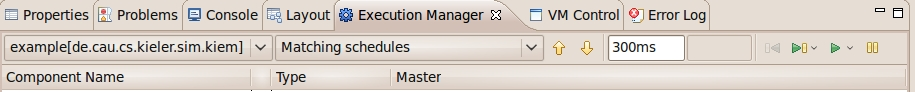
\includegraphics[scale=.4]{ToolbarWithContributions.jpg}
  \caption[The Execution Managers Tool bar with two contributed ComboBoxes]%
  {The Execution Managers Tool bar with two contributed ComboBoxes\protect}
  \label{fig:ToolbarWithContributions}
\end{figure}
\begin{figure}[H]
  \centering
  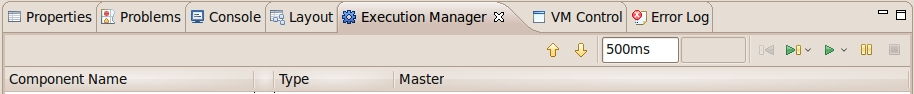
\includegraphics[scale=.4]{ToolbarWithoutContributions.jpg}
  \caption[The Execution Managers Tool bar without contributions]%
  {The Execution Managers Tool bar without contributions\protect}
  \label{fig:ToolbarWithoutContributions}
\end{figure}

\subsection{Configuration Provider}
\label{section:ConfigurationProvider}
\index{Configuration Provider}
\listingjava
\showlistingex{code/IKiemConfigurationProvider.txt}
{Java}
{The Interface of the Configuration Provider}
{list:IKiemConfigurationProvider}
{t}
The purpose of the configuration provider is to allow internal attributes of the
Execution Manager to be stored in another plug in. 

This is achieved by another extension point to allow any plug-in to listen to changes
in the Execution Manager's attributes. It also means that there may be multiple
plug-ins that provide values for properties and not all plug-ins may have the value for
a property needed by the Execution Manager. Through the plug-in mechanism the \ac{KIEM}
can ask all providers for values and choose the one he would like to use.

The two methods from the interface shown in Listing \ref{list:IKiemConfigurationProvider} work
in the following way:

\begin{description}
 \item \textbf{String changeProperty(String propertyId) throws KiemPropertyException} :

This method will be called by the Execution Manager whenever a property has to be loaded where
other plug-ins are encouraged to provide their value. When a plug-in is asked for a value it
can do one of two things:
 \begin{enumerate}
  \item It can either provide a value for the property. Any value is acceptable here, even \textit{null}.
If one plug-in provides any value at all the other plug-ins will not be asked. The reason behind this arrangement
is that the Execution Manager most likely can't decide which value has more validity anyway if more than one
plug-in answers.
  \item If it can not provide a value the declared Exception should be thrown in which case the Execution
Manager will move to the next plug-in. The reason for not using the \textit{null} value to encode no valid value
is that \textit{null} might be the intended value.
 \end{enumerate}

 \item \textbf{void propertyChanged(String propertyId, String value)} :

Notifies all listeners that a property was changed somewhere in the Execution Manager. This will be called for example
when the user changes the step duration through the input field on the Execution Managers tool bar.
\end{description}

\subsection{Event Listener}
\label{section:EventListener}
\index{Event Listener}
\listingjava
\showlistingex{code/IKiemEventListener.txt}
{Java}
{The Interface of the Event Listener}
{list:IKiemEventListener}
{t}
The main purpose of the Event Manager is to inform DataComponents of events
happening in the Execution Manager during execution. This behavior has been modified to include 
events that occur while the execution is not running. This modification lead to the 
creation of another extension point in order to allow other plug-ins to be notified
on any of these events as well. The classes implementing the interface 
(see List \ref{list:IKiemEventListener}) required by this extension point will be notified
on any event that happens inside the Execution Manager.

\begin{description}
 \item \textbf{int provideEventOfInterest()} : This method is directly derived from the method with 
the same name in the AbstractDataComponent class of the \ac{KIEM} plug-in. It is called by the
EventManager to determine which events the implementing class is interested in.
This is done to improve efficiency and not flooding components with events they are not interested in.

Based on the response, the EventManager puts the component into lists along with the DataComponentWrappers
already inside.
 \item \textbf{void notifyEvent(KiemEvent event)} : This method is called by the EventManager when 
something happens inside the Execution Manager that the implementing classes might be interested in.
\end{description}

\section{KIEMPlugin.java}
\label{section:ConfChangesKiemPlugin}
The main Activator class contains almost the entire \ac{API} of the \ac{KIEM}.
Therefore any additions to that has to performed in this class which means that
most of the adjustments were made here.

\subsection{Listener}
The following methods were added to communicate with the plug-ins registered through
the ConfigurationProvider extension point (see Section \ref{section:ConfigurationProvider}).
\begin{description}
 \item \textbf{notifyConfigurationProviders(String propertyId, String value)} : 

This method can be called by any class
inside the Execution Manager itself. It should be called when the user changes a property through any of
the elements on the \ac{GUI}. The method will then inform all listeners that the property identified by the
given identifier was changed to the new value.
 \item \textbf{String getPropertyValueFromProviders(String propertyId)} : 

This method allows the Execution Manager to
retrieve a previously saved value. The \ac{KIEM} will ask all plug-ins registered on the extension point if they
can provide a value for the given identifier. Plug-ins that can't provide the value will indicate this by throwing
an Exception. The \ac{KIEM} will then take the first value he receives without getting an Exception and assign it
to the internal property.
 \item \textbf{Integer getIntegerValueFromProviders(final String propertyId)} : 

This method is a convenience method for
the one described above. It will try to parse an integer from the retrieved String and return it or return null
if no integer could be parsed.
\end{description}

\subsection{Getters and Setters}
\listingjava
\showlistingex{code/getterSetter.txt}
{Java}
{Example of modified Getter and Setter}
{list:getterAndSetter}
{t}
An example for the use of the methods described in the last section can be found in the Getters and Setters for
the different properties in the Execution Manager (for an example see Figure \ref{list:getterAndSetter}). 
These were changed in order to use the new methods but are
still able to fall back on hard-coded default values if no configuration plug-in is registered.


\subsection{Open File}
\label{section:ConfKiemOpenFile}
\listingjava
\showlistingex{code/openFile.txt}
{Java}
{The head of the modified openFile() method}
{list:openFileMethod}
{t}
The method that takes care of loading an execution file was split. This was done to allow
other plug-ins to pass an IPath object directly to the method and perform a load of that file without
having to go through the \ac{UI}. This method was also shifted around a little in order to detect
missing execution files before the load enters the \ac{UI}Thread. This was necessary to make is possible for
the callers of the method to catch the resulting exception.
The method also had to be modified in order to be able to take files that are not inside the workspace
but were added through an extension point. The changed part of the openFile method is shown in 
Listing \ref{list:openFileMethod}.
The last change to that method concerns the event listener. When the user opens a file through the
Eclipse workspace without using the \ac{KIEMConfig} plug-in the plug-in still has to be informed.
This happens through the use of the Event Manager that notifies all listeners upon the successful
completion of the loading operation.


\section{KIEMView}
\label{section:ConfChangesKiemView}
The changes described in Section \ref{section:ConfChangesKiemPlugin} were mostly concerned with the
configuration management and loading of new execution files. This section will mostly deal with the changes
that were necessary to enable the adding of new items to the tool bar.

The tool bar of the Execution Manager is created in a programmatic way instead of through the use of the
corresponding Eclipse extension point. This means that the only way to place additional controls onto the tool bar
is to modify the code in order to make use of the Toolbar Contribution Provider extension point described
in Section \ref{section:ToolbarContributionProvider}. For the full code of the modified method see the
Appendix.

\chapter{The KIEMConfig plug-in}
\label{chapter:KiemConfig}
This chapter describes the contents and functionality of the newly created
plug-in to solve the problems described in Chapter \ref{chapter:ConfTask}.
A new plug-in was created in order to improve modularity within the \ac{KIELER} framework.
Putting the code into the \ac{KIEM} plug-in itself would have meant that
there would have been no way to separate the two projects.

The sections in this chapter describe the different parts of the \ac{KIEMConfig} plug-in.
The whole plug-in is structured according to the Model-View-Controller pattern.
The first section will describe the data storing classes which constitute the model.
The second section will describe the different manager classes which are essentially the
controller of the entire plug-in. This section will also look at the \ac{API} that the
\ac{KIEMConfig} plug-in provides to other plug-ins.
The last section will describe the classes that render the preference pages and other
view elements.

\section{Data Classes and Utilities - the Model}
\label{section:ConfModel}
This section will describe the different classes that are responsible for storing all
data that the plug-in needs at runtime.


\subsection{ConfigDataComponent}
\label{section:ConfigDataComponent}
\index{ConfigDataComponent}
This extension to the AbstractDataComponent of the \ac{KIEM} is responsible for solving
the problem described in Section \ref{section:ConfTaskConfig} and implements the behavior
described in Section \ref{section:ConfConceptsConf}. The component is a DataComponent
like all others used in the \ac{KIEM}. It is registered through the extension point
that allows new DataComponents to appear in the list of available components.
However unlike the usual DataComponent that is responsible for simulating a model during
an execution run its main function is to store the configuration of the \ac{KIEM}.

Like all other DataComponents the ConfigDataComponent contains an array of
KIEMProperties. These properties contain a String key which should be non-null and unique and 
a value which can be of various types. However for the purpose of storing configuration
elements only the String value will be used.

The new DataComponent also provides additional methods in order to make accessing and manipulating the
array more convenient:
\begin{description}
 \item \textbf{KiemProperty findProperty(String key)} : This method iterates through the array and attempts
to find the KiemProperty that has exactly the provided key. Since the keys are assumed to be unique the first
match is returned by this method. If there is no property with the given key the method will throw
an Exception.
 \item \textbf{void removeProperty(String key)} : This method attempts to remove the property identified by
the given key from the array. It does this by converting the array to a list, locating and removing the
specified property and then converting the list back to an array. This procedure may not be as efficient
as manually constructing the new array but it still performs the operation in linear time. Furthermore
it makes the method easier to understand than the alternative.
 \item \textbf{KiemProperty updateProperty(String key, String value)} : This method updates the property 
identified by the key with a new value. It first checks if the property already exists and if it does its value
is updated. If a property with the specified key doesn't exist a new one is created and the provided value
stored inside.
\end{description}

In addition to those methods the ConfigDataComponent also keeps a reference to its DataComponentWrapper (see Section
\ref{section:IntroDataComponentWrapper}). This is necessary in order to retrieve the properties from the wrapper
right after the execution file was loaded and to write them back into the wrapper before the file is saved.

The ConfigDataComponent is not only used to store the properties of the currently active configuration that each
execution file carries. However it is also used to store the default configuration that is saved in the Eclipse
preference store. This is done because both instances are closely linked and have the same requirements
(see Section \ref{section:CurrentConfiguration}).

The default behavior of the Configuration Manager is to add a new ConfigDataComponent to each execution file
that it encounters. However as this feature can be turned off the user also has can upgrade old files or
downgrade new ones by manually adding and removing the ConfigDataComponent.


\subsection{EditorDefinition}
\label{section:EditorDefinition}
\index{EditorDefinition}
The EditorDefinition class is responsible for storing information about the editors that are known to
the \ac{KIEMConfig}. Each instance of this class stores the information about a single editor. This is
necessary in order to successfully operate a list of execution files that work for the currently active
editor.
\begin{description}
 \item \textbf{String editorId} : The identifier for the given editor. This attribute is a unique non-null String
by which any editor can be identified. For example the standard Java editor has the id \textit{org.eclipse.jdt.ui.CompilationUnitEditor}.
 \item \textbf{String name} : The name of the editor. This is the human readable name given to the editor
by the plug-in that defines the editor. Storing this attribute may seem redundant since the names of
the editors can be retrieved through an Eclipse mechanism if the editor id is known. However there is no
guarantee that a previously saved editor id exists in the currently active application in which case the name
of the editor can't be retrieved.
 \item \textbf{boolean isLocked} : This attribute is responsible for showing that the editor can not be removed.
The reason that an editor might become read only will be explained in Section \ref{section:DefaultSchedule}.
\end{description}

\subsection{ScheduleData}
\label{section:ScheduleData}
\index{ScheduleData}
The ScheduleData class is responsible for tracking the different execution files that are known
to the \ac{KIEMConfig}. A ScheduleData object is the representation of a single execution file. 
These objects are used to main he lists of recently used schedules and of those that match the 
currently opened editor. It contains the following attributes:
\begin{itemize}
 \item The most important attribute is the path at which the execution file that this instance
should represent is located. The path is used to trigger the loading of the file inside
the Execution Manager. It is also used to determine whether a newly loaded execution file
is already known. The path also doubles as the unique identifier for the schedule since there
can't be two files at the same physical location.
\item The ScheduleData object also stores a list of priorities for all known editors. This is
necessary in order to determine whether or not a given schedule can be used with the currently
opened editor and which position it should have in an ordered list. To make accessing and manipulating
this list easier it simply uses an instance of the ConfigDataComponent. The component already has
methods for accessing the array inside and can be easily stored and loaded.
 \item Like the EditorDescription a ScheduleData also contains a boolean \textbf{isLocked}. ScheduleData
object with that attribute set to \textit{true} can't be modified or removed (see Section \ref{section:DefaultSchedule}).
\end{itemize}

\subsection{Tools}
\label{section:Tools}
The Tools class holds a host of useful methods and attributes that are used in various parts of the plug-in.

\subsubsection{Attributes}
\label{section:ToolsAttributes}
First of all it contains messages and tool tips that are used in more than one class.
This ensures that the appearance of the different messages is unified across the entire plug-in. It also
makes it easy to change these messages or combine different partial messages to new ones.

The class also holds the different identifiers for the properties that are used in the plug-in. This is done
to avoid bugs due to mistyping an identifier which is likely to happen if it is stored in two different places.

\subsubsection{Methods for Parsing and Serialization}
\label{section:ToolsMethodsParsing}
All of the manager classes in the \ac{KIEMConfig} need to save their properties into the Eclipse preference store.
In order to have the information stored in a structured way an \ac{XML} like format was chosen. As this requires the keys and values
to be formatted in a certain way the Tools class provides methods to format the Strings in the required way.
\lstset{
backgroundcolor=,
}
\begin{description}
 \item \textbf{String putValue(String key, String value} : Converts the (key, value) pair into a formatted String for saving
into the Eclipse preference store. The resulting String has the following format: 
\lstinline|<[key]>[value]</[key]>|.
 \item \textbf{String putProperty(KiemProperty property} : Convenience method for transforming a KiemProperty object into a
formatted String. This method exists because most of the items serialized in this way are of that type. The resulting String
has the following format: \lstinline|<KIEM_PROPERTY><Key>[property.key]</Key><Value>[property.value]</Value></KIEM_PROPERTY>|.
\end{description}

The methods described above provide all the necessary facilities for the \ac{KIEMConfig} to save its preferences
into the Eclipse preference store. In order to retrieve these properties the Tools class provides another set of
methods. These methods take an input String and try to parse the saved properties.
\begin{description}
 \item \textbf{String getValue(String key, String input)} : This method retrieves the value enclosed by tags with
the given key. The retrieved value can either be an atomic String that can directly be assigned to a property or
another series of values enclosed in their tags. The method will always look for the outermost tags inside the
input String. The method returns null if there are no tags with the provided key inside the input String.
 \item \textbf{KiemProperty getKiemProperty(String input)} : This convenience method tries to retrieve the 
(key, value) pair that constitutes a KiemProperty object from an input String.
 \item \textbf{String[] getValueList(String key, String input)} : Since there sometimes is the need to store an entire
list of entities the Tools class provides a method to convert an entire list back to the individual Strings.
The method iterates over the input String and extracts all elements that are enclosed in tags with the specified key.
\end{description}


\subsubsection{Methods for Dialogs}
\label{section:ToolsMethodsDialogs}
The Tools class also contains methods for easily displaying error and warning dialogs.
These methods take the information, add the own plug-in id and forward the information to the 
error handling facilities inside the Execution Manager itself.


\subsection{MostRecentCollection}
\label{section:MostRecentCollection}
The MostRecentCollection is a new collection type that is can be used for simulating the 
behavior found in 'Open recent' menu item of almost any text editing application.
To avoid the list growing too long it can be given a maximum capacity. After that capacity
is reached the oldest entry will be deleted when a new one enters the list.
The default implementation of the collection uses an ArrayList to store the data but any
other list works as well. Most operations are directly delegating to the operations of the 
underlying List. 
The only exception is the add(item : T) method that works in a different way:
\begin{enumerate}
 \item It checks if the item is already in the list and removes it. This is done to ensure
that already added items don't appear twice in the list.
 \item It adds the item at the highest index to the end of the list and increments the index of all other items.
 \item The element at the head of the list is overridden by the new item.
 \item Optionally the last item is removed if the list has grown beyond the capacity.
\end{enumerate}
The collection also provides an additional method that is used to replace an item in
the list by another one. This is used when files are renamed and the name of the ScheduleData inside
the list has to be updated.

This collection is used to track the most recently used schedules and display them
in the corresponding ComboBox.



\section{Manager Class - the Controller}
\label{section:ConfController}
The manager classes are responsible for the control flow inside the plug-in. They gather information
from the view, the Eclipse preference store and the Execution Manager and create and update a
model using the classes described in Section \ref{section:ConfModel}. There are multiple managers
each with a different task:
\begin{itemize}
 \item The \textbf{Configuration Manager} is responsible for maintaining the configuration saved in
each execution file and the default configuration saved in the preferences store.
 \item The \textbf{Schedule Manager} is responsible for keeping track of the different
execution files and updating the information inside the ScheduleData objects.
 \item The task of the \textbf{Editor Manager} is to
\end{itemize}



\subsection{Abstract Manager}
\label{section:AbstractManager}
All of the managers share some common features that each of them must provide. Some of those
features are handled almost the same or exactly the same in each manager. This lead to the creation
of an abstract super class for all managers (see Figure  %\ref{fig:AbstractManagerUML}) 
that takes care of the basic tasks.

The first task is to allow other classes to register as a listener to the manager. Some of the classes
in the \ac{KIEMConfig} have to perform updates when a value inside the model changes. It is the managers
responsibility to inform the listeners when such a change was completed successfully.

The second task is to provide the subclasses with facilities to easily access the Eclipse Preference Store.
Whenever a value is requested by any part of the controller or another plug-in and a manager didn't access
the preference store yet it has to gain access to the store and retrieve the information belonging to it.
Furthermore when the user explicitly wants to save the preferences or the workbench is shutting down the
data contained in the model has to be saved into the Eclipse Preference Store. For an example of a 
saved configuration see the Appendix.


\subsection{Configuration Manager}
\label{section:ConfigurationManager}
\index{Configuration Manager}
The Configuration Manager basically handles all the problems described in Section \ref{section:ConfTaskConfig}.
This means that the Configuration Manager has two responsibilities:
\begin{enumerate}
 \item It manages the configuration contained in the currently opened execution file and all properties contained in
it. It is also responsible for deciding whether or not the preferences stored in that configuration should be used
or the default preferences instead.
 \item It manages the default configuration that the user can access and modify through the preference pages 
(see Section \ref{section:ConfView}). For all of the predefined properties it also has to hold and manage the 
hard-coded default values.
\end{enumerate}

\subsubsection{Currently Loaded Configuration}
\label{section:CurrentConfiguration}
\index{Current Configuration}
The first thing the Configuration Manager has to do when a request for the value of a property is made
is to locate the ConfigDataComponent that contains the property. 

It first takes a look at the list of keys where the default configuration should be used. If this is the case the task is quite simple
and the default configuration is loaded from the preference store and used. If the current configuration
should be used the task is a little more difficult. The Configuration Manager then has to look at the
DataComponentWrapperList inside the Execution Manager where all components for the currently opened
execution file are stored. If the list already contains a wrapper with the ConfigDataComponent inside
that component is used. Otherwise a new ConfigDataComponent is created, initialized with the default values
from the default configuration and then added to the list of the current execution file. Since this feature
can be disabled by the user the Configuration Manager can encounter execution files that have no ConfigDataComponent
or where the component simply doesn't contain the requested value. In this case the default configuration has
to be used.

If the default configuration couldn't supply a value the last possibility is that the caller passed a non-null default 
value for the given property. In this case the default value is returned to the caller. 

If no value could be retrieved in the way described above there is no way to get a valid value for the requested key. 
In this case the Configuration Manager notifies the caller through an exception of these circumstances.

However if the value was expected in the current configuration but not found the Configuration Manager assumes 
that it should have been in there. To remedy that situation the Configuration Manager will try to add a new property 
to the current configuration with the value that the method will return (either the one retrieved from the default 
configuration or the default supplied by the caller).


\subsubsection{Default Configuration}
\label{section:DefaultConfiguration}
\index{Default Configuration}

The first responsibility of the Configuration Manager with respects to the default configuration is to manage
the hard-coded default values. The whole idea of the \ac{KIEMConfig} is to avoid using hard-coded values
and retrieve user defined values. However the Execution Manager and the \ac{KIEMConfig} rely on certain values
to be present and even though the user is encouraged to change them they still have to be present before the user
enters them for the first time. Furthermore the user may want to revert back to sensible default values which
should be provided by the plug-in itself.

This means that the plug-in contains a list of hard-coded default values for the needed properties.
It also supplies methods to access these properties and restore the default values by writing their values
into the default configuration.

\lstset{
backgroundcolor=,
}
The next feature that the default configuration supplies has to do with adding new ConfigDataComponents to the
list inside the Execution Manager. Since the Configuration Manager knows which properties will be taken from
the current configuration it can already make sure that the component contains some value. This is done
through calling \lstinline|void initWithDefaults(AbstractDataComponent dataComponent)| with the newly created component.
This causes the default values for all properties that are likely to be taken from the current configuration to
be added to it.

The Configuration Manager also supplies different views on the default configuration. 
\begin{enumerate}
 \item \textbf{KiemProperty[] getDefaultConfig().getProperties()} : This method simply returns all properties
stored in the default configuration. This is the list actually written to the Eclipse preference store.
 \item \textbf{KiemProperty[] getInternalDefaultProperties()} : This method returns the list of properties that
are needed to operate the Execution Manager and the \ac{KIEMConfig}. The motivation for this method is that
the keys and types for these values are already known. That means that a view that modifies these properties
can be designed in a more user-friendly way than would have been possible otherwise. Furthermore the Configuration 
Manager is guaranteed to have hard-coded default values for these properties.
 \item \textbf{KiemProperty[] getExternalDefaultProperties()} : This method returns the complement of the internal
properties with respect to the entirety of the default properties. These properties are those that the user defined
himself.
\end{enumerate}
However neither of the last two lists will return the default editor as that falls into the responsibility of
the Editor Manager which is described below.

The Configuration Manager also supplies methods to add new properties to the default configuration, remove properties
and update the value of specific property.

\subsection{Schedule Manager}
\label{section:ScheduleManager}
\index{Schedule Manager}
The Schedule Manager is the second of the two large managers. It is responsible for managing the
ScheduleData object, the execution files and provide the methods for solving the problem described
in Section \ref{section:ConfTaskEasyLoading}. These responsibilities can be broken down into
six different parts:
\begin{enumerate}
 \item Gather the different types of lists of schedules.
 \item Manage the different ScheduleData objects and provide methods to add, remove and change
them.
 \item Deal with loads and saves triggered through the normal workspace interface.
 \item Provide a means to trigger the loading of an execution file in the Execution Manager.
 \item Track the locations of the execution files if the user modifies them.
 \item Loading the default schedules.
\end{enumerate}


\subsubsection{Provide the Schedule Lists}
\label{section:ProvideScheduleLists}
The Schedule Manager stores all ScheduleData objects in one list that is saved and loaded through
the abstract super class. However different components of the \ac{KIEMConfig} or other plug-ins 
need different views on that list. Some components may not want to display all schedules or have
the list sorted in a certain way. To provide these different views the Schedule Manager contains
several methods:
\begin{description}
 \item \textbf{List<ScheduleData> getAllSchedules()} : Returns the list of all schedules. This
method triggers a load through the super class if no load has been performed yet. It also triggers
a load of the default schedules described at the end of Section \ref{section:DefaultSchedule}.
 \item \textbf{List<ScheduleData> getMatchingSchedules(String editorID, String editorName)} :
This method is responsible for constructing the list that will be displayed in the ComboBox that
shows the list of schedules matching the currently active editor. First it tries to find an
EditorDefinition with the given editor id. If that fails a new EditorDefinition is created and
added it to the list of known editors. After that the method searches through the list of
all schedules and extracts those that have a positive priority for the given editor. The list
is then sorted  and returned with the editor with the highest priority appearing at the lowest index.
 \item \textbf{List<ScheduleData> getRecentSchedules()} : This method constructs the list of 
recently used schedules. This list is used in another ComboBox to allow the user to easily load
his last used schedules. In order to realize this feature the Schedule Manager keeps a list of
all execution file locations that were recently accessed using the list described in Section
\ref{section:MostRecentCollection}. When the method is called it iterates over the list of locations
and tries to find a schedule for each location. Schedules that match a location in that list are 
added to the resulting list. Entries in the list of locations where no schedule can be found will
be removed from the list as they are no longer valid.
 \item \textbf{List<ScheduleData> getImportedSchedules()} : Returns the list of default schedules.
This feature will be described in detail at the end of Section \ref{section:DefaultSchedule}.
\end{description}


\subsubsection{Listen to User Events}
\label{section:UserEvents}
It has to be assumed that the user creates his own schedules and saves and loads them through the workspace explorer.
Since the Schedule Manager should attempt to track all available execution files it has to be informed about
these changes and act on the notification. In order to get notified the Event Listener extension point
of the Execution Manager is used (see Section \ref{section:EventListener}). The listener will dispatch and event
that contains the location of any saved or loaded execution file as soon as the user performs the corresponding action.
When the Schedule Manager receives such an event it will perform the following steps:
\begin{enumerate}
 \item Try to find a schedule with the provided location. If a schedule can be found there is nothing to be
done and the method skips to the last step.
 \item If no schedule was found with the given location a new one has to created. In order for that the method
first has to check if there is an active editor and if the editor is known to the Schedule Manager. If that is
the case the method skips ahead to step 4.
 \item If the editor is unknown it is created. If no editor is active the default editor will be used.
 \item The new schedule is created with the editor determined in the previous steps. Since it is assumed that
the created schedule works with the currently active editor a default priority is inside to that editor in the
newly created schedule.
 \item Since the file operation constitutes a use of the given schedule the list of recently used schedules has
to be updated. The used schedule will be added to the top or moved to the top if it's already inside.
\end{enumerate}


\subsubsection{Open a Schedule}
\label{section:OpenSchedule}
The Schedule Manager also provides a way to trigger a load in the Execution Manager. This is
done through the modified method described in Section \ref{section:ConfKiemOpenFile}. The reason for this
is that the Schedule Manager may try to load schedules where the files no longer exist or that the 
Execution Manager is unable to load. The method mentioned above will throw Exceptions in order to perform
the caller of these circumstances and the Schedule Manager will inform its callers.

As described in the last section the Schedule Manager will be informed of a load through the Event Listener
interface and will act on it. However if the load is triggered by the Schedule Manager itself that behavior
would not be desirable. To avoid the Schedule Manager informing itself the method makes sure that the next
event indicating a loaded file will be ignored.

Since the load triggered by the Schedule Manager constitutes an access to that file the associated schedule
is added to the list of recently used schedules. Furthermore all listeners on the Schedule Manager will
be notified since view updates may be necessary.


\subsubsection{Tracking Execution Files}
\label{section:TrackingExecutionFiles}
As described above new schedules will be created when the user manually loads or saved an execution file.
However in some cases the user may also choose to remove, rename or move execution files. Since the Schedule Manager
relies on the path of the execution file to load the schedules it runs into trouble if the path is changed outside
its control.

The only solution in this case is to prompt the user to select a new path for an execution file that is no
longer at the expected location. An alternative would be to simply delete the schedule and all assigned priorities.

\lstset{
backgroundcolor=,
}

However if the user performs a remove, rename or move through the context menu inside the Eclipse workspace window
Eclipse itself provides a way to get notified of these changes. Any class can register themselves as listener
by calling : 
\lstinline|RefactoringCore.getHistoryService().addHistoryListener(IRefactoringHistoryListener listener)|.
Whenever the removal, renaming or moving of a file completes all listeners will be notified through a call to
\lstinline|void historyNotification(RefactoringHistoryEvent event)|. The event contains different information
based on the type of the operation. Depending on the type of operation that was performed the Schedule Manager
takes one of the following actions:
\begin{description}
 \item \textbf{Delete} : One or more files were deleted by the user. In this case the event contains the list
of files that was deleted. Since the user has no more use for the deleted files he probably has no use for
the schedule and the saved priorities as well. The Schedule Manager attempts to find the ScheduleData object
associated with the given file and removes it.
 \item \textbf{Rename} : The user changed the name of a file. The event provides the old file name and the 
new name of the file. In order to keep track of the file the Schedule Manager tries to find the ScheduleData
associated with the old file name and changes the name to the new file.
 \item \textbf{Move} : One or more files were moved by the user to a new location. The event contains the list
of files that were moved and the destination path. The Schedule Manager tries to find a Schedule for each
of the files involved and changes its name to reflect the new location.
\end{description}


\subsubsection{Default Schedule}
\label{section:DefaultSchedule}
\index{Default Schedule}
\index{Extension point}
An additional requirement that came up through the development of this project was that it would
be desirable to provide the user with an initial set of execution files that are not located inside
the users workspace.

For that purpose the new extension point seen in Listing \ref{list:DefaultSchedule} was created.
\listingxml
\showlistingex{code/defaultSchedule.txt}
{XML}
{Example implementation of the Default Schedule extension point.}
{list:DefaultSchedule}
{t}

As soon as the Schedule Manager loads the schedules from the Eclipse preference store it also triggers
a load from the components registered on this extension point. The new schedule will be constructed with
the location provided through the corresponding field in the extension point. After that the Schedule Manager
iterates through the list of child elements of a given execution file and adds all the editors and their
priorities to the schedule and the Editor Manager.

Since the schedules and editors added in this way are supposed to be a kind of factory defaults they are not
supposed to be removed or changed. The Schedule Manager sets a field in both the newly created ScheduleData
objects and the EditorDefinitions. It is the responsibility of the different view elements not to modify
entities marked in this way.


\subsection{Editor Manager}
\label{section:EditorManager}
\index{Editor Manager}
As described in Section \ref{section:EditorDefinition} the editor names and editor ids have to be saved
since they might not be available in the current runtime environment. The Editor Manager is responsible
for managing the list of all known editors. It also contains facilities around the default editor.

\begin{description}
 \item \textbf{EditorDefinition addEditor(EditorDefinition editor} : Adds a new editor to list of 
editors and return the added editor. If an editor with that editor id already exists in the list it is
not added to prevent duplicates. In this case the already existing editor is returned instead. Since
some methods may want to work on the editor that was just added they can work on the returned reference
instead of having to perform a find to get the correct object.
 \item \textbf{EditorDefinition findEditorById(String id)} : This method searches through the list
of available editors to retrieve the editor with the given id. Since editors ids are assumed to be
unique the first match is returned. This method is for example used to build the list of schedules that
work with the currently active editor.
 \item \textbf{void removeEditor(EditorDefinition editor)} : At some point the user may decide that
one of the editors is no longer used. In this case the editor is simply removed from the list of
available editors. However if the removed editor is the default editor (see Section \ref{section:DefaultEditor})
the method also has to choose a new default editor. The editor of choice for simplicity is the first
editor in the list. If the last editor is removed a hard-coded default editor is restored.
\end{description}

When the user is finished changing the editors the manager can use the facilities in the super class to
write the list of known editors to the Eclipse preference store.


\subsubsection{Default Editor}
\label{section:DefaultEditor}
\index{Default Editor}
The \ac{KIEMConfig} contains a facility for showing the list of schedules that match the currently active
editor. However there may be situations no editor is opened. Since the user should be able to keep working
with his schedules in this situation there is the need to define a default editor. This editor will be assumed open 
when in fact no editor is active.

Although the actual storing of the default editor happens inside the Configuration Manager the Editor Manager
still supplies facilities to get and set the default editor. This arrangement is more intuitive than having
the methods inside the Configuration Manager.


\subsection{Contribution Manager}
\label{section:ContributionManager}
\index{Contribution Manager}
The Contribution Manager is responsible for maintaining the view elements (see Section \ref{section:ScheduleSelector}) 
that are not part of any of the preference pages. To accomplish this the manager has two tasks:
\begin{enumerate}
 \item The manager must create the view elements and store them. As described in Section 
\ref{section:ToolbarContributionProvider} the Execution Manager will ask the \ac{KIEMConfig}
for the list of items it wants to contribute to the tool bar. The manager then has to 
create the list with the saved view elements and forward it through the extension point.
 \item As the user might want to hide the new elements the Contribution Manager also has to 
keep track of the visibility of the elements. Showing and hiding the components is realized
in the following way:
\begin{itemize}
 \item When the Execution Manager requests the list of control contributions the Contribution Manager
checks whether or not the given view element should be visible. If it should not be shown on the tool bar
it is not added to the list and thus never reaches the tool bar.
 \item When the user changes the visibility of a given view element the manager first updates its own
representation of that information and triggers a save into the Eclipse preference store through the use
of the facilities in the super class. After that the manager triggers a refresh in the Execution Manager
view which causes the method in the extension point to be called which then receives the changed list.
\end{itemize}
\end{enumerate}


\subsection{Property Usage Manager}
\label{section:Property Usage Manager}
\index{Property Usage Manager}
As described in Section \ref{section:ConfTaskDefaultConfig} the user might not want to use
the properties saved in the currently loaded execution file but rather the default values
entered through the preference page. The Property Usage Manager is responsible enabling
the Configuration Manager to realize this feature.

To accomplish this task the manager contains a list of property keys for those values
that should be taken from the default configuration. The list can be changed by any other
class when the user changes the preferences on which properties should be in it. The list
is also stored and loaded through the use of the facilities in the Abstract Manager.


\section{Preference Pages - the View}
\label{section:ConfView}
The view part of this project mostly consists of the preference pages for setting up the different
aspects of the \ac{KIEMConfig}. These preference pages use the technology described in Section
\ref{section:TechPreferencePage} which integrates them into the rest of the preference page
framework. The root page for the Execution Manager is added into the already existing tree
of preference pages for the rest of \ac{KIELER} in order to make them easier to find.

\subsection{Configuration Page}
\label{section:ConfigurationPage}
\index{Configuration Page}
\begin{figure}
  \centering
  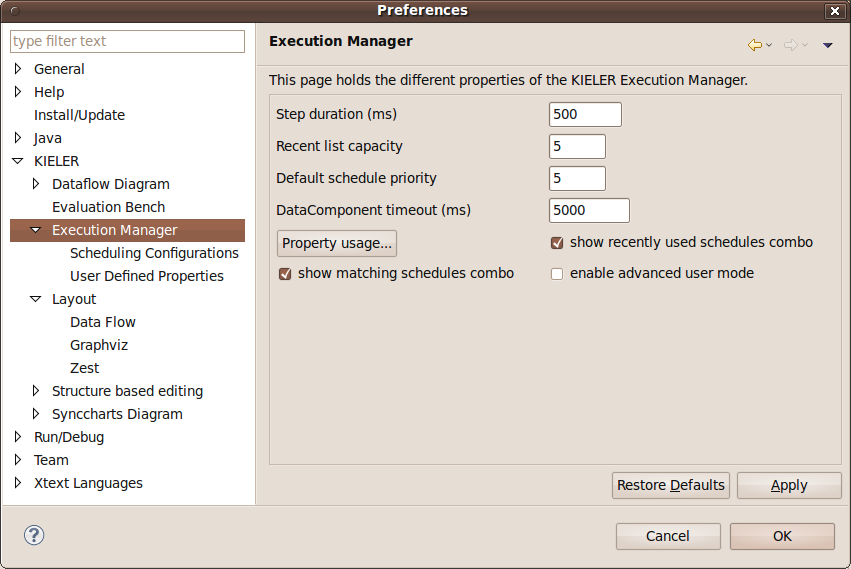
\includegraphics[scale=.4]{ConfigurationPage.png}
  \caption[The main preference page of the Execution Manager]%
  {The main preference page of the Execution Manager\protect}
  \label{fig:ConfigurationPage}
\end{figure}
On the main preference page of the Execution Manager shown in Figure \ref{fig:ConfigurationPage} the user can
set up most of the default properties. The user can also change the visibility of the ComboBoxes that display
the recently used and matching schedules. The last CheckBox is for enabling the advanced user mode.

In the normal user mode the ConfigDataComponent described in Section \ref{section:ConfigDataComponent} is
not visible to the user. It is also automatically added to any new file that is loaded into the Execution Manager.
While this behavior is fine for the average user an advanced user may want to have a little more control. An advantage
of having the component visible is that the user can reinitialize the current configuration with the values in
the default configuration by removing and adding the component in the list.


\subsubsection{User-Defined Properties Page}
\label{section:UserDefinedPropertiesPage}
\begin{figure}
  \centering
  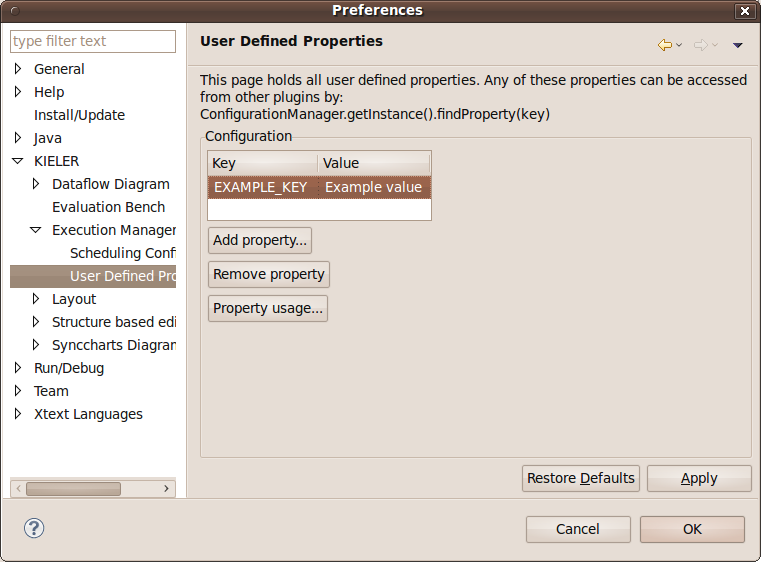
\includegraphics[scale=.4]{UserPropertiesPage.png}
  \caption[The page for defining custom properties]%
  {The page for defining custom properties\protect}
  \label{fig:UserDefinedPropertiesPage}
\end{figure}
Since there is a page to modify the internal properties of the Execution Manager there also exists a
preference page where the user can define, edit and remove his own properties (see Figure \ref{fig:UserDefinedPropertiesPage}). 
These properties can then be accessed by any DataComponent (or any other plug-in) through the \ac{KIEMConfig}'s \ac{API}.

Since not much can be said about the nature of the user defined properties there is no real format that
can be chosen for an individual property. Thus all properties are simply displayed in a table with a 
key and a value column. 

The user is only allowed to edit the value column of previously defined properties. This restriction is
necessary to keep the user from accidentally changing keys that are required by another users DataComponent.

However the user can remove a property that is no longer needed or define his own properties with a custom key.

\subsubsection{Property Usage Dialog}
Both of the previously described pages contain a button for accessing the Property Usage Dialog.
This dialog (see figure \ref{fig:PropertyUsageDialog}) is used for selecting which properties should always be taken
from the default configuration rather than the configuration component contained in every .execution file.
The dialog used for this is a ListSelectionDialog which just receives the list of
all keys as input and the list of PropertyKeys from the PropertyUsageManager as default selection.
After the user is finished with selecting attributes and hit the 'Ok' Button the dialog
passes the new list of selected items back to the PropertyUsageManager.
\begin{figure}
  \centering
  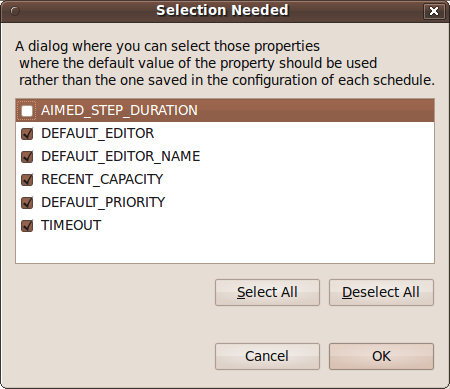
\includegraphics[scale=.4]{PropertyUsageDialog.png}
  \caption[Property Usage Dialog]%
  {The Property Usage Dialog\protect}
  \label{fig:PropertyUsageDialog}
\end{figure}

\subsection{Scheduling Page}
\label{section:SchedulingPage}
\index{Scheduling Page}
\begin{figure}
  \centering
  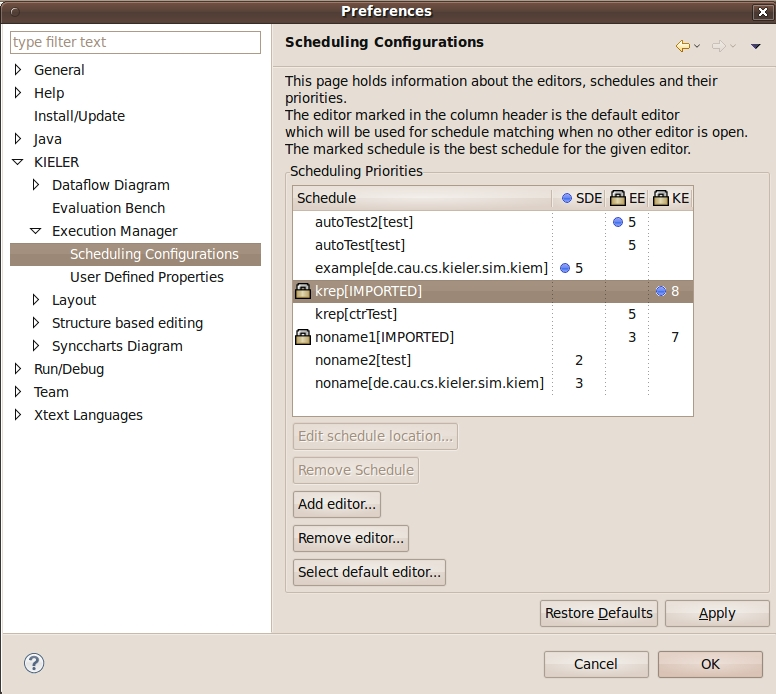
\includegraphics[scale=.4]{SchedulePage.jpg}
  \caption[The page for managing the schedules and editors]%
  {The page for managing the schedules and editors\protect}
  \label{fig:SchedulePage}
\end{figure}
This preference page (see Figure \ref{fig:SchedulePage} is used to manage the schedules and the editors that they belong to.
As mentioned in Section \ref{section:ConfConceptsDefaultConf} this page is basically a modified version 
of the LayoutPrioritiesPage by Miro Sp\"onemann (see Figure \ref{fig:MSPLayoutPreferencePage}).

The page is divided into two parts. The top part shows the table, the bottom part the buttons for manipulating
the table entries.

The table column headers show the abbreviated names of the editors (the tool tip of each header will show the full name). 
Each column represents the priorities that the different schedules have for this particular editor. When the editor is
active in the workbench view the list of matching schedules will be sorted in the order of these priorities. The user
can directly edit these properties in the table. For easier readability the best schedule for each editor is marked
with a dot and the table is sortable by clicking any of the column headers.

The editors and schedules that have a padlock next to their name are the ones imported through the default schedule 
extension point described in Section \ref{section:DefaultSchedule}. These editors and schedules are not supposed
to be edited or removed since they represent a factory default setting. The view realizes this by graying out the 
corresponding buttons when an imported schedule is selected.

All other schedules can be removed by simply clicking the appropriate button. The button for editing the location
of a schedule opens a dialog showing the currently active workspace and allows the user to select a new
execution file that should be associated with the selected schedule. This feature is necessary in case the user
moves a schedule through his file browser instead of the refactoring facilities on the workbench.

The editor marked with the dot is the default editor (see Section \ref{section:DefaultEditor}.

\subsubsection{Adding and Removing Editors, Selecting a Default Editor}
\begin{figure}
  \centering
  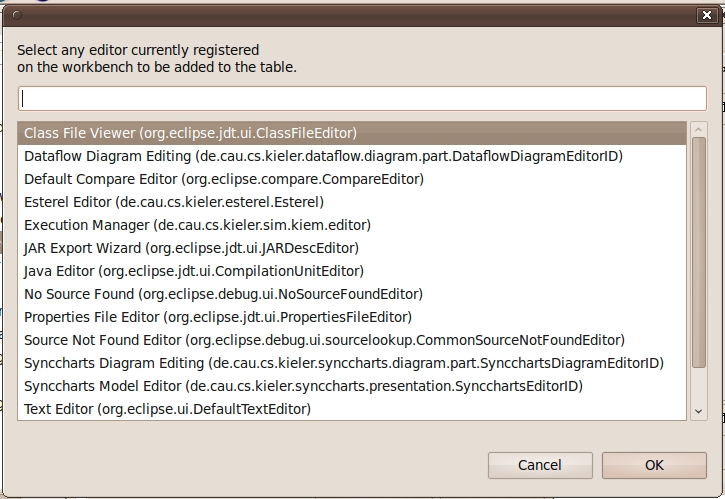
\includegraphics[scale=.4]{EditorSelectionDialog.jpg}
  \caption[Editor Selection Dialog]%
  {The Editor Selection Dialog\protect}
  \label{fig:EditorSelectionDialog}
\end{figure}

On the scheduling preference page there are routines for adding and removing
editors as well as selecting a default editor.
All of these actions use the same basic method for displaying an ElementListSelectionDialog \ref{fig:EditorSelectionDialog}
that takes a list of editor ids and returns the one selected by the user.
\begin{itemize}
 \item The editor adding dialog gets a list of all editors currently registered on the
 active workbench. The user can select a single editor which is then added to the table.
 \item The editor removal dialog gets a list of all editors currently available for 
 assignment of support properties. The editor selected by the user is removed from the table.
 It is also removed from all schedules. This is done to prevent the schedule objects from growing
 to unnecessarily large size over time when editors are getting added and removed.
 \item The default editor selection dialog gets the same list as the removal dialog. The selected
 editor is then set as default editor. 
\end{itemize}


\subsection{Schedule Selector}
\label{section:ScheduleSelector}
\index{Schedule Selector}
\begin{figure}
  \centering
  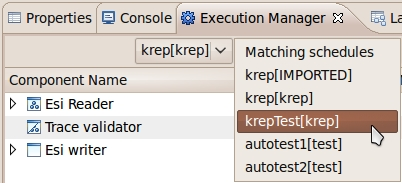
\includegraphics[scale=.4]{ScheduleSelector.jpg}
  \caption[The Schedule Selection ComboBoxes]%
  {The Schedule Selection ComboBoxes\protect}
  \label{fig:ScheduleSelector}
\end{figure}
The Schedule Selector is the only view element isn't shown on the preference pages. It is used
to construct and manage the two ComboBoxes for loading schedules that are known to
the \ac{KIEMConfig}. Each of the two ComboBoxes seen in Figure \ref{fig:ScheduleSelector} has its own task.
\begin{description}
 \item \textbf{The Matching Selector} : This ComboBox displays the schedules that can be used with
the currently active editor. The list is sorted by the priorities assigned through the preference page.
It displays a header showing its purpose in order to distinguish it from the other ComboBox.
 \item \textbf{The Recently Used Selector} : This ComboBox displays the list of recently used schedules.
The list is ordered in the same order that the schedules have been accessed through the Execution Manager.
The maximum size of the list can be configured through the preference page. The ComboBox displays the name
of the currently loaded execution file regardless of how it was loaded. This was done because up till now 
there actually was no way to tell which execution file was loaded in the Execution Manager.
\end{description}


\chapter{Conclusion}
\label{chapter:ConfConclusion}
As stated in Chapter \ref{chapter:ConfTask} the problem consists of two parts:
\begin{enumerate}
 \item Find a way to add configurations to the existing execution files. Additionally find
a way to allow the user the set up default preferences.
 \item Make it easier to load previously saved schedules without having to locate
the execution file in the workspace.
\end{enumerate}
The following sections will summarize the results and provide some ideas for
future work.

\section{Results}
The first task was to implement a way for execution files to carry configuration
properties. This was solved by creating a new type of DataComponent that stores all
properties and is accessed by the \ac{KIEMConfig} when values for the properties are needed.
The newly created component is automatically saved with any execution file that wants to
use the new feature.

Part of the first task involved enabling the user to manage a default configuration
for the different properties. This was realized through the creation of a set
of preference pages. These pages allow the user to manage the properties and even
override the ones stored in the execution file.

The last objective concerned the actual loading of the execution files. A way had to be
found in order to make loading the files easier and provide filtered perspectives on all known
files. This was accomplished by providing the user with two ComboBoxes that contained a
subset of all known execution files. One ComboBox is used to load the most recently used files
while the user contains files that probably work for the currently active editor.

\section{Future Work}
Although all initial goals of this thesis were more than met there are still
some features that could not be added due to the lack of time.
\subsection{Eclipse Runtime Mechanism}
The Eclipse framework provides a very comprehensive system to run different
modules. This is used to execute Java programs or to start a new Eclipse application
but there are a variety of other applications as well.

The entire Execution Manager could be refactored into using that runtime mechanism instead
of setting up a run through the now present \ac{KIEM} view. This means that the table
that shows the DataComponents has to be moved to a new runtime page. 

The controls for pausing, resuming, stopping and stepping through the execution have to
be moved somewhere else as well, possibly the DataTable.

\subsection{Improve Storage Options}
Currently DataComponents as well as the preference mechanism only allow the use of
Strings to store the preferences. This means that all primitive data types can more
or less be stored by conversion to a String. However more complex objects can't be stored
without serializing them into a String and parsing them again on load.

A future project could try to find a way to overcome that limitation by allowing
objects that implement the \textit{Serialization} interface to be stored as well.

\subsection{Use Advanced KiemPropertyTypes}
Currently the \ac{KIEMConfig} can only handle KiemProperties of the basic type that
contains a String value. However there is a whole range of different KiemPropertyTypes
such as integer, files or choice. An enhancement to the \ac{KIEMConfig} would be to
utilize the full potential of these types.

This would mean rewriting much of the already existing code and completely refining
the page where the user can define their properties.

\section{Summary}
All in all the initial problem of providing a means to storing additional configuration information
in an execution file as well as providing a mechanism for providing a default configuration was solved. 
In addition to that the second objective which involved finding a way to make it easier to load previously
saved schedules was also completed.

However there is still a lot of basic for further work on the concepts of this project and on the
concept of the Execution Manager in general.

\part{Automated Execution}
\chapter{Used Technologies}
\label{chapter:AutoTechnologies}

In addition to the technologies used in the first part of this
thesis (see Chapter \ref{chapter:ConfTechnology}) other Eclipse
technologies will be used as well.

The next sections will describe the technologies and give some
examples of their usage in the standard Eclipse application.
The technologies described here are the following:
\begin{description}
 \item The Job: The Eclipse Job is a mechanism for very long running tasks.
 \item The Wizard: The wizard is a method for helping the user to set up complex tasks.
\end{description}


\section{The Job}
\label{section:AutoTechJob}

The Eclipse Job \ac{API} provides the means to schedule very long running tasks.
It uses a Thread to run the actual task and contains a ProgressMonitor to show
the progress of the task. Since it is a task that can run independently of the
current state of the workspace it can also be run in the back ground if the user
desires it.
An example for the use of jobs in the normal Eclipse architecture
is the SVN commit operation seen in Figure \ref{fig:SVNCommit}.

\begin{figure}[SVNCommit]
  \centering
  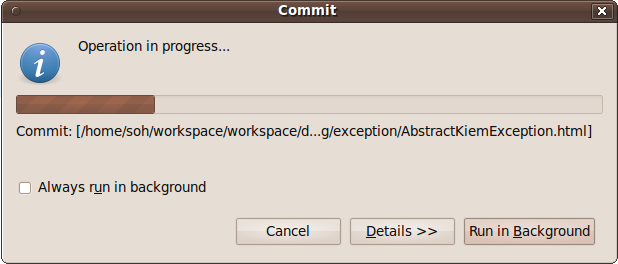
\includegraphics[scale=.4]{SVNCommit.png}
  \caption[The SVN commit job]%
  {The SVN commit job\protect}
  \label{fig:SVNCommit}
\end{figure}

\section{Eclipse Wizards}
\label{section:AutoTechWizards}
Wizards are used to guide the user through the process of creating complex items by taking
the information in a structured way and then generating the item from it.
One example inside the Eclipse Architecture is the Java Class Creation Wizard (see Figure \ref{fig:ClassWizard})
In theory it is possible to open a text file and enter all the information manually.
However if the wizard is used the user only has to select the class he wants to extend
and the interfaces he wants to implement, activate one check box and then the wizard will
create the class body, all required methods and comments for each element (see Listing \ref{fig:classCreationGenerated})
This makes it very easy for even inexperienced users to create new classes without knowing
the exact syntax.

\begin{figure}[ClassWizard]
  \centering
  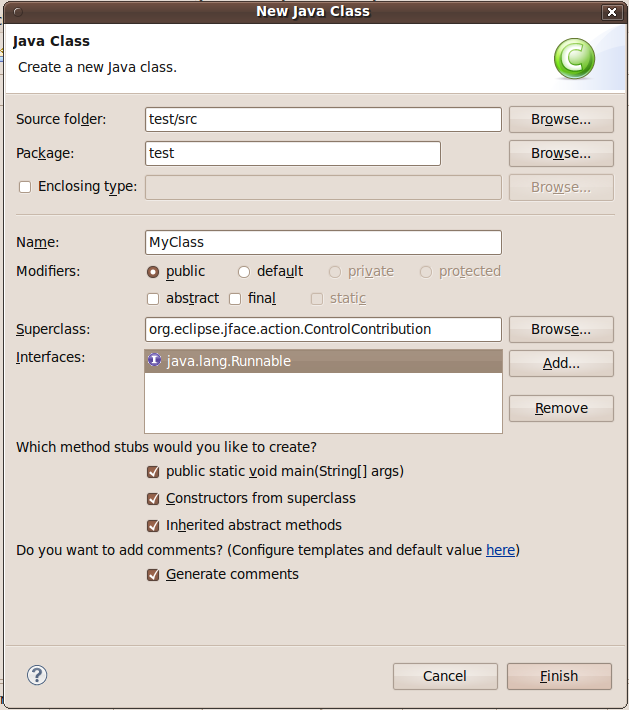
\includegraphics[scale=.4]{ClassWizard.png}
  \caption[The Class Creation Wizard]%
  {The Class Creation Wizard\protect}
  \label{fig:ClassWizard}
\end{figure}

\lstset{
  language=Java,
  frame=shadowbox, 
  rulesepcolor=\color{blue},
  caption=Code generated by the wizard,
  label=fig:classCreationGenerated,
}
\begin{lstlisting}
package test;

import org.eclipse.jface.action.ControlContribution;
import org.eclipse.swt.widgets.Composite;
import org.eclipse.swt.widgets.Control;

public class MyClass extends ControlContribution 
   implements Runnable {

   /**
    * Creates a new MyClass.java.
    * 
    * @param id
    */
   public MyClass(String id) {
      super(id);
   }

   /**
    * {@inheritDoc}
    */
   @Override
   protected Control createControl(Composite parent) {
      return null;
   }

   /**
    * {@inheritDoc}
    */
   public void run() {
   }

   /**
    * @param args
    */
   public static void main(String[] args) {
   }
}
\end{lstlisting}


\chapter{Problem Statement}
\label{chapter:AutoTask}

In order to do validations or recording automatically in a batch-like mode, 
the Execution Manager needs to be extended by an Eclipse Plug-in that some kind of 
remote controls it (API) and has/supports for example: 
\begin{itemize}
 \item An own eclipse view (GUI) 
 \item Loading and saving batch files 
 \item Some way to specify batch jobs (e.g., a special notation language) 
 \item Possibly a way to do all this from the command line
\end{itemize}


Currently the KIEM works in a way that you select an execution file and then
press play. The components then have to gather all information they need
themselves like model files, trace files and so on. The execution runs until
the user or a component stops it. The user then has to manually set up another
execution run, possibly even rewriting his components if the model files
and trace files are hard coded.
This is very unsatisfactory if you have a large number of model files that
should be tested with a one or more execution files and several trace files.
% ask ctr for screenshot of directory perhaps

The problem can be broken down in 4 parts which are explained in detail in
the following sections:
\begin{enumerate}
 \item The setup of an automated run by the user.
 \item The input of all the necessary information.
 \item The control flow of the automated run.
 \item The gathering of information after the run has finished and the display 
of that information.
\end{enumerate}


\section{Setting up a Run}
\label{section:AutoTaskSetup}
The first objective is to find an easy way for the user to efficiently set up an
automated run. This involves selecting the model files and execution files
needed for the automation as well as entering initial properties.

\section{Input for the Automation}
\label{section:AutoTaskInput}
The second objective is to enable the components to receive inputs.
Each component should receive all information it needs prior to each execution
run in order to make the components more dynamic. This mechanism would ensure
that components can be written in a more generic way than is currently possible.
We will have to define an API for this information passing process as well as
an API to trigger an automated execution from other plug-ins.


\section{Automate the execution}
\label{section:AutoTaskExecution}
The third objective is to automate the process of execution itself. This would
involve the following:
\begin{enumerate}
  \item loading an execution file
  \item stepping the execution to the required step
  \item gather the information produced by the components
  \item properly shut down the execution so that a new one can be started
\end{enumerate}


\section{Output execution results}
\label{section:AutoTaskOutput}
The last objective is to display the information in a meaningful way.
This should involve at least two methods of output:
\begin{enumerate}
  \item A formatted string possibly in an XML fashion that can be parsed and
  used by other plug-ins for automatic analysis.
  \item Some graphic component that will display the information in way that is
  easy to read for most users.
\end{enumerate}


\chapter{Concepts}
\label{chapter:AutoConcepts}

\section{Setting up a Run}
\label{section:AutoConceptsSetup}
There are several possibilities of how to solve the problem of accumulating
large amounts of information prior to a long running action.
The first possibility would be to have the user enter the paths to the 
necessary files in text files, parse those files and start a run with
the parsed information. While this is a good method for performing
static runs from a console environment it has several disadvantages
inside the \ac{GUI} of an Eclipse \ac{RCA}:
\begin{itemize}
 \item Manually entered file names in a text file are prone to have erroneous information.
It is very hard to manually enter the correct file name of any file and the entered location
only works on one \ac{OS}. Aside from that it takes a long time to manually enter the possible vast
amount of files used.
 \item There is no way to quickly adjust the file if other models or execution files should be used.
 \item It also means more files cluttering up the workspace.
 \item It is not very intuitive and the user has to know the exact syntax that the execution needs.
\end{itemize}

Another approach is the selection of the files through a dialog.
Here the first option is to write a new dialog from scratch. While this option
ensures flexibility since only the elements that are really needed are on it in
exactly the way they are needed some disadvantages come along:
\begin{itemize}
 \item It involves a lot of work since every widget has to be manually placed on the dialog.
 \item It involves even more work to get the layout of the dialog just right.
\end{itemize}

A more comprehensive approach would be to use one of the dialogs provided by Eclipse specifically the wizard type dialog.
Eclipse itself uses a host of wizards as explained in Section \ref{section:AutoTechWizards}.
The wizard has several advantages over the other methods explained here:
\begin{itemize}
 \item Even inexperienced users can be guided to set up a valid execution run.
 \item The entered information is most likely valid since the wizard only displays valid files.
 \item It is quicker to program and easier to adjust than any of the other methods.
\end{itemize}


\section{Input for the Automation}
\label{section:AutoConceptsInput}
In order to send information to the DataComponents (see Section \ref{section:IntroDataComponent})
the first decision must consider the form of the information that will be supplied.
The chosen form is that of a list of (key, value) pairs. It allows for most
flexibility while still being very generic and simple to read and write on.
This list of properties will at least include the path to the model file (see Section \ref{section:IntroModelFile}) in order
for components to be executed with several different model files without having
to alter the code between runs.

The next decision involves how the components are getting the information.The first possibility 
would be to have the component ask the plug-in for the information
in question. The upside of this would be that components are sure to get all the information
they need before the execution can start since they can keep asking for it. However this would
likely mean that the component has to poll multiple times as it has no knowledge about when
the required information will be available which constitutes additional workload. Furthermore
this situation would likely mean that multiple components might request information
at the same time. This means that there would be the need for substantial synchronization mechanisms
to ensure consistency of data.

Therefore the way chosen in this thesis is that the Execution Manager will inform interested components
about all properties that were accumulated and then starts the execution run. This ensures
that a run is started in any event and keeps communication between the components and the manager simple.

\section{Automate the execution}
\label{section:AutoConceptsExecution}
Automating the execution itself requires the plug-in to interact with the Execution Manager.
There is already an \ac{API} defined for loading an execution file by supplying a path so that
is what will be used in this project.
Then it is necessary to initialize the execution and step through it using the \ac{API}
methods provided in the Execution Manager. For this the EventListener extension point (see Section \ref{section:EventListener}) of the 
Execution Manager can also be used in order to determine when a step has finished executing and
a new one can be dispatched.
After the execution is finished all components should be called again to be given
a chance to provide information for the display in the next step. This information
will be gathered in the same form and way as described in Section \ref{section:AutoConceptsInput}.


\section{Output execution results}
\label{section:AutoConceptsOutput}
On the subject of displaying the information several options are available.

The first option would be to open a dialog once the execution has finished
and display the results in a tabular manner. This has the advantage that the
users attention is immediately caught when the run finishes. However pop-up boxes
should be used only when something very important happens and only with small messages
as they tend to interrupt the users work flow. Aside from that the user might want
to look at the results from the execution and compare them with the actual model.
An opened dialog is usually something sitting in front of the rest of the \ac{IDE}
and that user wants to get rid of as fast as possible.

The option taken in this project will utilize the view mechanism provided by Eclipse. %ref to description of view
This approach ensures that the user can place the displayed results where he wants them to be.
It also makes it possible for the user to run an execution multiple times and compare the
results by having them displayed in multiple views or next to each other in the same view.
Another advantage of the view concept is that it provides a tool bar for adding actions.
The user might want to control the automated run during its execution or interact with
the displayed results. While a static dialog would have difficulties providing the control elements
for those actions a view can easily display them in the tool bar.

\chapter{Code changes in KIEMPlugin}
\label{chapter:AutoKiemChanges}
\begin{itemize}
 \item interfaces and API changes to allow access to execution
 \item changes to load values rather than hard coded defaults
\end{itemize}

\section{Schema files and Interfaces}
\begin{itemize}
 \item event listener mentioned in part I, for listening to KIEM execution
 events
 \item interfaces added to KIEM itself to avoid components breaking when
 automated plug-in is not loaded
\end{itemize}

\chapter{The Automated Executions Plug-in}
- new plugin
- handles the setup, control flow and display of automated execution
- consists of 3 parts explained in detail below
- wizard, manager, view

\section{Automated Component}
An automated component is any DataComponent that wants to interact with
the automated execution plug-in. As seen in the diagram automated components
have to implement three methods:

\subsection{provideProperties()}
This method enables components to receive information prior to each execution
run. The list is implemented as an array of key, value pairs stored inside
KiemProperty objects.
At the every least the list contains the location of the model file and the
index of the currently running iteration (that is how many time the current
model has already been executed with the current execution file).
This allows components to load additional files that are always in the
same path as the execution file and determine which of those to load
based on the iteration index.

\subsection{wantAnotherStep()}
This method is called after every step of the execution manager.
All components are asked if they want to perform another step and if
one components answers with TRUE the execution manager will perform another
step.
This makes it unnecessary to know the exact number of steps needed for
the execution before the execution starts.

\subsection{wantsAnotherRun()}
This method is the equivalent for the wantAnotherStep() method in the context
of entire execution runs.
After no component wants to perform another step all components are asked
if they want to perform another run. If one component answers with TRUE
the entire simulation is stopped and then started again with the same
model file and execution file but an incremented iteration index.
This can for example be used to execute the same model with a different
set of trace files by just naming the trace files the same way as the
model files with a number at the end.

\section{Automated Producer}
This interface extends the AutomatedComponent interface.
In addition to the inherited methods it provided one additional method.
This method is called after an iteration has finished and asks the components
if they want to publish any information about the results of their execution.
This information is gathered by the plug-in and the accumulated results
are either passed to the calling plug-in or displayed in the
specially designed view (see chapter about the view).

\section{Automation Wizard}
\subsection{File Selection Page}
- wizard is used to set up the execution run
- extends ResourceImportWizard for displaying a folder/file structure for selecting files from
- easily usuable, select whole folders, filter file types
- can be given an initial selection, on close will save the selection, store it in preference store
and restore it on load
- additional dialog for selecting execution files that are not in the workspace but imported
- for simplicity assume that files ending .execution are execution files and all other selected
ones are model files, wizard can not check if valid since formats are not known
- only allow user to proceed if at least one execution and one model file is selected
\subsection{Property Setting Page}
- set up the additional arguments passed to the execution
- simple adding and removing of key, value pairs
- same as file page, on close results are saved to preference store and restored for initial
selection on next open
\subsection{Information Processing}
- gather execution files and model files from file selection page
- gather properties from property page
- store information for next open
- invoke the execution manager

\section{Automation manager and Automation Job}
- handles control flow during the automation
- takes information from either call through the API or wizard

\subsection{Automation Manager}
- handles the overall control flow
- takes the execution files, model files and properties as argument
- if progress monitor is registered it is informed about the progress of the evaluation
- The control flow:
\begin{itemize}
 \item iterate over all execution files
 \item open execution file
 \item tell view to set up display for the first execution file
 \item iterate over all model files
 \item get first model file from list
 \item ask components how many more runs they need, take maximum and perform runs before asking again
 \item pass model file, execution file and index of iteration
 \item initialize the execution
 \item pass properties to components, at least receive model file and iteration
 \item start worker thread that listens for monitor canceling, step timing out
 \item ask components how many more steps they need, take maximum and perform steps before asking again
 \item perform one step, lock self inside semaphore, stay locked until either worker thread or event listener notifies (step done)
 \item when no component wants more steps pause
 \item gather information from all IAutomatedProducers
 \item tell view to show information for this iteration
 \item stop execution inside the KIEM and perform cleanup
 \item proceed to next iteration
 \item inform monitor of progress
 \item proceed to next model
 \item proceed to next execution
 \item when done inform monitor of done and terminate the job
\end{itemize}



\subsection{Automation Job}
- workbenchjob with progressmonitor
- used to display the progress in the progress view and a dialog with progress bar
- long running task, doesn't want to block the rest of the workbench 
- triggers execution in the manager

\section{Automation View}
- displays the information in a structured way
- start a new table for each execution file
- one row for each iteration with each model file
 - prerequisite needed here: always the same outputs throughout the entire execution file
- first columns display model file name, iteration index and current status

\subsection{Toolbar}
- button to start the wizard
- button for clearing the view
- text field showing the step that was just processed

\chapter{Conclusion}
\label{chapter:AutoConclusion}
As stated in Chapter \ref{chapter:AutoTask} the problem consists of four parts:
\begin{enumerate}
 \item Find an easy way for the user to set up an automated run.
 \item Input the information provided by the user into the data components.
 \item Design a control flow for an automated run.
 \item Organize the output of the automated run and display it to the user.
\end{enumerate}
The following sections will summarize the results and provide some ideas for
future work.

\section{Results}
\label{section:AutoResults}
The first objective of the project was to solve the set up of an automated run
by the user. The initial idea of using a script-based approach and providing the
necessary files as lists in text files was not pursued. Instead a more user-friendly
solution was found through the use of a wizard. 

The next objective was to find a way to input information into the DataComponents
in order for them to be designed in a more generic way. This was achieved by
designing new interfaces that allow components to receive a list of properties
prior to each part of the automated execution.

The main part of the task involved creating a manager that guided the control flow
of an automated execution. The Automation Manager described in Section \ref{section:AutomationManager}
loads all the necessary files, sets up the different outputs, steps through the
execution to the desired step and includes error management facilities as well.

The last part was to find a user-friendly way to display the information generated
by the automated execution. The problem was solved by creating a view that displayed
the information in a set of tables. These tables are structured in a way to easily
compare the results of different model files and iterations. To allow use of the 
generated tables in another context methods were implemented in order to allow
the generation of external formats (namely \ac{CSV} and \LaTeX).


\section{Future Work}
\label{section:AutoImprovements}
Although all initial objectives were achieved there is still room for additional
improvements. These improvements which could be the subject of further study will
be explained in this section.

\subsection{Scripting}
Currently the automated execution can be triggered through
the use of a wizard and will run inside the Eclipse workbench and display the results
in a graphical view. 

In order to allow other plug-ins or external applications to trigger
an automated execution an interface would have to be defined. This could involve the 
creation of a scripting language that passes all the needed parameters to the automated
execution. It would also involve retrieving those results and importing them into the 
calling application.

The existing code already supports most of the requested features however there is no
interface to access those features from outside of Java.

\subsection{Exports}
Currently the only possibility to use the collected data in
another application is by exporting the entire table into \ac{CSV} or \LaTeX .

This process could be improved, for example by allowing the user to select the table columns
and rows that he wants to export instead of exporting the entire table. Furthermore
export to additional formats could be implemented. It could even be possible to interface
the entire automation with a database application or remote system.

\section{Summary}
All in all the initial problem of providing a framework for setting up automated execution runs
was solved. 

Further testing and use of these features may however reveal new ways that the
plug-in can extend its functionality.



\setcounter{secnumdepth}{0}
\appendix

\backmatter
\appendix
\chapter{Appendix}
\label{chapter:AppendixA}
\listingjava
\showlistingex{code/toolbarCode.txt}
{Java}
{Example for the use of extension point code in the modified creation of the Execution Manager's tool bar.}
{list:AppendixToolbarCode}
{H}
\label{chapter:AppendixB}
\listingxml
\showlistingex{code/savedPreferences.txt}
{XML}
{Example for a configuration saved into the Eclipse preference store}
{list:AppendixSavedConf}
{H}

%
\printglossary

%%% Local Variables: 
%%% mode: latex
%%% TeX-master: "paper"
%%% End: 


\printindex            

%%% Local Variables: 
%%% mode: latex
%%% TeX-master: "paper"
%%% End: 

\begin{thebibliography}{cmot-dt}
 \bibitem{cmot-dt}Christian Motika, Semantics and Execution of
 Domain Specific Models, 2009.
 \bibitem{eclipseOverview}Object Technology International, Inc. Eclipse Platform Technical Overview,
2003.
 \bibitem{eclipsePlugins}Eric Clayberg and Dan Rubel. Eclipse Plug-ins. Addison Wesley, 2009.
\end{thebibliography}

%\chapter{Bedienungsanleitung}\index{Bedienungsanleitung}
Um mit der Uhr arbeiten zu k"onnen muss man als erstes eine Batterie
einlegen. Die Uhr wechselt dann sofort in den Macrozustand \zst{alive}, und
dort in den Unterzustand \zst{displays}. Von nun an werden Sekunden Minuten
und Stunden auf dem LCD-Display angezeigt. 


\begin{description}
\item[Dr"ucken von \kn{Knopf d}:]
M"ochte der Benutzer der Uhr sich nun  das datum ausgeben lassen, dann dr"uckt
er den \kn{Knopf d}. Die Uhr wechselt nun in den Zustand \zst{date} und das 
Datum
erscheint auf der LCD-Anzeige. 

\item[Dr"ucken von \kn{Knopf a}:]
Um in das uhr-Men"u zu gelangen muss man nur den \kn{Knopf a} dr"ucken. 
Folgende mehrfachbenutzung ist m"oglich:
\begin{description}
\item[Bei einfachem Dr"ucken von\kn{ Knopf a}]
gelangt man in das Men"u von Alarm1. Mit Hilfe des \kn{Knopfes d} wird der 
Alarm1
in den Zustand \zst{on} oder durch erneutes Dr"ucken in den Zustand  \zst{off}
geschaltet. 
Befindet sich der Alarm1 im Zustand \zst{on}, dann erscheint eine kleine
Glocke mit einer 1  oben links in der Ecke der Uhr. 
Befindet sich nun der Alarm1 im Zustand \zst{off}, dann erlischt die kleine
Glocke wieder. 

Um den Alarm zu stellen muss der Benutzer den \kn{Knopf c} dr"ucken. Nun kann 
man mit dem \kn{Knopf d} die Stunden erh"ohen. Ist die gew"unschte einstellung
vorgenommen, dann gelangt man "uber das dr"ucken von \kn{Knopf c} zum Stellen 
der Zehnerstelle der Minuten. Nach fertigem einstellen gelangt man wieder "uber
einen Druck auf \kn{Knopf c} zum Stellen der Minuten. Sind nun alle 
Einstellungen vorgenommen worden, dann gelangt man mit Hilfe des 
\kn{Knopfes c} zur"uch ins Men"u von Alarm1. 
Um wieder in den \zst{time}-Zustand zu gelangen, in dem die Uhrzeit
angezeigt wird muss man noch viermal den Knopf a dr"ucken. 

\item[Bei zweifachem Dr"ucken von \kn{Knopf a}]
gelangt man in das Men"u von Alarm2. Das Men"u von Alarm2 ist genauso
aufgebaut, wie das Men"u von Alarm1 (s.o.). Mit der ausnahme, dass man beim
verlassen des Zustandes durch dreifaches Dr"ucken in den Zustand \zst{time}
gelangt. 
 
\item[Bei dreifachem Dr"ucken von \kn{Knopf a}]
gelangt man in das Men"u des Zustands \zst{Chime}. Mit Hilfe des \kn{Knopfes d}
kann man nun einstellen, dass die Uhr alle volle Stunde einmal  alarm schlagen
soll. Durch erneutes Dr"ucken des Knopfes d wird diese Funktion wieder
ausgeschaltet. Ist der Zustand \zst{Chime} aktiv, dann erscheint auf dem
Uhr-\eng{display} eine kleine gelbe Glocke. Ist der Zustand inaktiv, dann 
erlischt sie wieder.  
Um wieder in den \zst{time}-Zustand zu gelangen muss man noch zweimal den 
Knopf a dr"ucken. 

\item[Bei vierfachem Dr"ucken von Knopf a] gelangt man in das Stopuhr-Men"u.
  Die LCD-Anzeige erweitert sich automatisch um die M"oglichkeit nun auch \cs
  anzeigen zu k"onnen. Durch das Dr"ucken von \kn{Knopf c} startet man die 
Stopuhr. Um nun die Zeit zu stoppen gen"ugt ein erneutes Dr"ucken des 
\kn{Knopfes c}.  M"ochte man die Stopuhr wieder auf Null setzen, dann muss 
man den \kn{Knopf d}  dr"ucken.  In den Zustand \zst{time} gelangt man durch 
einfaches Dr"ucken  von \kn{Knopf a}.
\end{description}

\item[Dr"ucken von \kn{Knopf b}:]
Die LCD-Anzeigen Beleuchtung der Uhr erscheint durch das Dr"ucken von \kn{Knopf
b}. Wird nun nocheinmal dieser Knopf gedr"uckt, dann erlischt das Licht
wieder. 
\item[Batterie:]
Ist die Batterie der Uhr schwach (Das Signal \signal{Batt\_weakens} wird
emittiert), dann beginnt die Uhr zu blinken. Wird die Batterie
herausgenommen oder erlischt, dann bleibt die Uhr stehen. 
\end{description}

%%% Local Variables: 
%%% mode: latex
%%% TeX-master: "paper"
%%% End: 




\end{document}

%%% Local Variables: 
%%% mode: pdflatex
%%% TeX-master: paper.tex
%%% End: 